%%%%%%%% ICML 2026 EXAMPLE LATEX SUBMISSION FILE %%%%%%%%%%%%%%%%%

\documentclass{article}

% Recommended, but optional, packages for figures and better typesetting:
\usepackage{microtype}
\usepackage{graphicx}
\usepackage{subcaption}
\usepackage{booktabs} % for professional tables

% hyperref makes hyperlinks in the resulting PDF.
% If your build breaks (sometimes temporarily if a hyperlink spans a page)
% please comment out the following usepackage line and replace
% \usepackage{icml2026} with \usepackage[nohyperref]{icml2026} above.
\usepackage{hyperref}

\usepackage{graphicx}
\usepackage{amssymb}
\usepackage{amsmath} 
\usepackage{multirow}
\usepackage{caption}
\usepackage{soul}  
\usepackage[normalem]{ulem}
\usepackage{makecell}
\usepackage{enumitem}
\usepackage{algorithm}
\usepackage{algpseudocode}
% \usepackage{algorithmic}
\usepackage{wrapfig}
\usepackage{subcaption}
\usepackage{paracol}   
\usepackage{booktabs}
% Attempt to make hyperref and algorithmic work together better:
% \newcommand{\theHalgorithm}{\arabic{algorithm}}
\newcommand{\fix}{\marginpar{FIX}}
\newcommand{\new}{\marginpar{NEW}}
\newcommand{\OurMethod}{NOCTA}
% Use the following line for the initial blind version submitted for review:
% \usepackage{icml2026}

% For preprint, use
\usepackage[preprint]{icml2026}

% If accepted, instead use the following line for the camera-ready submission:
% \usepackage[accepted]{icml2026}

\usepackage{amsmath}
\usepackage{amssymb}
\usepackage{mathtools}
\usepackage{amsthm}


% if you use cleveref..
\usepackage[capitalize,noabbrev]{cleveref}

%%%%%%%%%%%%%%%%%%%%%%%%%%%%%%%%
% THEOREMS
%%%%%%%%%%%%%%%%%%%%%%%%%%%%%%%%
\theoremstyle{plain}
\newtheorem{theorem}{Theorem}[section]
\newtheorem{proposition}[theorem]{Proposition}
\newtheorem{lemma}[theorem]{Lemma}
\newtheorem{corollary}[theorem]{Corollary}
\theoremstyle{definition}
\newtheorem{definition}[theorem]{Definition}
\newtheorem{assumption}[theorem]{Assumption}
\theoremstyle{remark}
\newtheorem{remark}[theorem]{Remark}

% Todonotes is useful during development; simply uncomment the next line
%    and comment out the line below the next line to turn off comments
%\usepackage[disable,textsize=tiny]{todonotes}
\usepackage[textsize=tiny]{todonotes}

% The \icmltitle you define below is probably too long as a header.
% Therefore, a short form for the running title is supplied here:
\icmltitlerunning{\OurMethod: Non-Greedy Objective Cost-Tradeoff Acquisition for Longitudinal Data}

\begin{document}

\twocolumn[
  \icmltitle{\OurMethod: Non-Greedy Objective Cost-Tradeoff \\ Acquisition for Longitudinal Data}

  % It is OKAY to include author information, even for blind submissions: the
  % style file will automatically remove it for you unless you've provided
  % the [accepted] option to the icml2026 package.

  % List of affiliations: The first argument should be a (short) identifier you
  % will use later to specify author affiliations Academic affiliations
  % should list Department, University, City, Region, Country Industry
  % affiliations should list Company, City, Region, Country

  % You can specify symbols, otherwise they are numbered in order. Ideally, you
  % should not use this facility. Affiliations will be numbered in order of
  % appearance and this is the preferred way.
  \icmlsetsymbol{equal}{*}

  \begin{icmlauthorlist}
    \icmlauthor{Dzung Dinh}{equal,unc}
    \icmlauthor{Boqi Chen}{equal,unc}
    \icmlauthor{Yunni Qu}{unc}
    \icmlauthor{Marc Niethammer}{ucsd}
    \icmlauthor{Junier Oliva}{unc}
    %\icmlauthor{}{sch}
    %\icmlauthor{}{sch}
  \end{icmlauthorlist}

  \icmlaffiliation{unc}{Department of Computer Science, UNC Chapel Hill}
  \icmlaffiliation{ucsd}{Department of Computer Science and Engineering,
University of California San Diego}
  % \icmlaffiliation{sch}{School of ZZZ, Institute of WWW, Location, Country}

  \icmlcorrespondingauthor{Dzung Dinh}{ddinh@cs.unc.edu}
  % \icmlcorrespondingauthor{Firstname2 Lastname2}{first2.last2@www.uk}

  % You may provide any keywords that you find helpful for describing your
  % paper; these are used to populate the "keywords" metadata in the PDF but
  % will not be shown in the document
  \icmlkeywords{Machine Learning, ICML}

  \vskip 0.3in
]

% this must go after the closing bracket ] following \twocolumn[ ...

% This command actually creates the footnote in the first column listing the
% affiliations and the copyright notice. The command takes one argument, which
% is text to display at the start of the footnote. The \icmlEqualContribution
% command is standard text for equal contribution. Remove it (just {}) if you
% do not need this facility.


% Use ONE of the following lines. DO NOT remove the command.
% If you have no special notice, KEEP empty braces:
% \printAffiliationsAndNotice{}  % no special notice (required even if empty)
% Or, if applicable, use the standard equal contribution text:
\printAffiliationsAndNotice{\icmlEqualContribution}

\begin{abstract}
% In many critical applications, resource constraints prevent observing all features at test time, motivating selective information acquisition for the predictions. For example, in healthcare, patient data spans diverse features ranging from lab tests to imaging studies, each may carry different information and must be acquired at a cost of time, money, or risk to the patient. Moreover, temporal prediction tasks, where both instance features and labels evolve over time, introduce additional complexity in deciding when or what information is important. 

In many critical domains, features are not freely available at inference time: each measurement may come with a cost of time, money, and risk. Longitudinal prediction further complicates this setting because both features and labels evolve over time, and missing measurements at earlier timepoints may become permanently unavailable. We propose \texttt{\OurMethod}, a \textbf{N}on-Greedy \textbf{O}bjective \textbf{C}ost-\textbf{T}radeoff \textbf{A}cquisition framework that sequentially acquires the most informative features at inference time while accounting for both temporal dynamics and acquisition cost. \texttt{\OurMethod} is driven by a novel objective, NOCT, which evaluates a candidate set of future feature-time acquisitions by its expected predictive loss together with its acquisition cost. Since NOCT depends on unobserved future trajectories at inference time, we develop \emph{two complementary} estimators: (i) \texttt{NOCT-Contrastive}, which learns an embedding of partial observations utilizing the induced distribution over future acquisitions, and (ii) \texttt{NOCT-Amortized}, which directly predicts NOCT for candidate plans with a neural network. Experiments on synthetic and real-world medical datasets demonstrate that both \texttt{\OurMethod} estimators outperform existing baselines, achieving higher accuracy at lower acquisition costs.
% than state-of-the-art baselines.

% We first introduce a cohesive estimation target for our \texttt{\OurMethod} setting, and then develop \emph{two complementary} estimators: 1) a \emph{non-parametric method} based on nearest neighbors to guide acquisitions (\texttt{\OurMethod-NP}), and 2) a \emph{parametric method} that directly predicts the utility of potential acquisitions (\texttt{\OurMethod-P}). Experiments on synthetic and real-world medical datasets demonstrate that both \texttt{\OurMethod} variants outperform existing baselines, achieving higher accuracy at lower acquisition costs.



\end{abstract}
\section{Introduction}
\label{intro}
% In many real-world scenarios, \textit{acquiring information is itself a decision}. 
In many real-world scenarios, \textit{the inference-time acquisition of information is a critical decision}. For example, in clinical settings (a driving application for this work), diagnostic decisions often rely on sequentially gathering information such as lab tests or imaging. Each type of data acquisition comes at a cost of time, financial expense, or risk to the patient. In contrast, standard supervised machine learning pipelines typically assume that \emph{all} features are freely available at inference.

In this work, we focus on \emph{longitudinal} Active Feature Acquisition (LAFA) \citep{saar2009active, kossen2022active}, where, during inference, a model is responsible for (i) sequentially deciding \emph{which features} to acquire and at \emph{what time}, balancing their utility against acquisition costs, and (ii) \emph{making predictions} with the partially observed features it has chosen to acquire.  In this setting, leveraging the temporal context is crucial for both selecting valuable feature acquisitions and making accurate predictions.
Fig.~\ref{fig:AFA_example} illustrates an example of LAFA by an autonomous agent in a clinical scenario. At the current visit, the agent 
% (1) reviews previously collected data alongside any measurement acquired at the current visit, (2) predicts the patient's status (label) at the current visit, and (3) recommends a date for future visit when more information is required for assessment and the tests to perform at that visit (accounting for acquisition costs).
(1) reviews previously collected data alongside any measurement acquired at the current visit, (2) predicts the patient's current status $\hat{y}_t$, and (3) decides when to schedule the next visit and which tests to acquire then (accounting for measurements' acquisition costs). Practical constraints such as time, cost, and resource limitations necessitate a judicious selection. 
%Between acquisition timepoints, the agent refines its predicted status using the data acquired so far.
Between visits, the agent continues to forecast the disease progression utilizing the previous acquisitions. 
% Because the agent cannot revisit earlier time points, 
% missed acquisitions in the past have become inaccessible. 

% % In particular, we focus on a \emph{longitudinal} setting where features may originate from diverse sources and data types, and long temporal contexts may be crucial for both selecting valuable acquisitions and making accurate predictions. 
% Fig.~\ref{fig:AFA_example} illustrates an example of longitudinal AFA methods driven by an autonomous agent operating in a clinical scenario. At the current visit, the agent \todo{[JO] tweak para, this is a critical description that should 100 percent match with our setting, and doesn't quite atm} (1) reviews previously collected data alongside any measurement acquired at the current visit, (2) predicts the patient's current status, and (3) recommends a future follow-up plan by specifying both the visit interval (e.g., 3 or 6 months) and the tests to perform at the visit, while accounting for acquisition costs. Although in principle a comprehensive set of tests could be performed, practical constraints such as time, cost, and resource limitations necessitate a more selective approach. Between visits, the agent projects the patient's trajectory to future time points, using the data acquired so far and the proposed time interval.
% % Between visits, the agent continues to forecast the disease progression based on the time elapsed. 
% Because the agent cannot revisit earlier time points, it must carefully decide whether to acquire information now or defer it, risking that missed acquisitions become permanently inaccessible. 
% % defer or perform tests at each time step to avoid missing potentially important acquisitions. 


\begin{figure}
    \centering
    
    % \includegraphics[width=0.82\linewidth,height=0.245\textheight, trim=0cm 0cm 0cm 0cm, 
    \includegraphics[width=1\linewidth,height=0.20\textheight, trim=0cm 0cm 0cm 0cm, 
clip]{figures/AFA_v4.pdf}
    \caption{Illustration of clinical longitudinal AFA. At the current visit, an autonomous agent reviews previously collected and newly acquired data, predicts the patient's current status, and recommends a subset of examinations for a determined future timepoint. This process repeats until the agent recommends no further acquisition.}
    \label{fig:AFA_example}
\end{figure}
% Challenges in AFA

This longitudinal AFA setting presents several challenges, including: deciding which features to acquire at each visit, facilitating early predictions for timely interventions, and accounting for temporal settings where missed acquisitions at earlier time points are permanently inaccessible. Although previous work has explored various approaches for longitudinal AFA, some methods~\citep{kossen2022active} make a single prediction across all time points, neglecting dynamic predictions, which are critical in clinical settings to detect deterioration early and adjust treatment plans \citep{qin2024risk}. Furthermore, recent reinforcement learning (RL)-based methods~\citep{qin2024risk,nguyen2024active} can be difficult to optimize in practice, while greedy strategies~\citep{gadgil2023estimating} risk suboptimal decisions because they focus on short-term gain and may skip early measurements that later prove critical but cannot be reacquired. This motivates non-greedy methods that are practical to train and deploy. \looseness=-1
% \todo{be clear about what's new about NOCTA when compared to prior methods}

\textbf{Contributions}\quad We propose \texttt{\OurMethod} (\textbf{N}on-Greedy \textbf{O}bjective \textbf{C}ost-\textbf{T}radeoff \textbf{A}cquisition), a non-greedy framework for longitudinal AFA that explicitly plans over future acquisitions without training an RL policy. \uline{First}, we introduce NOCT, the longitudinal objective underlying \texttt{NOCTA} that balances prediction accuracy against the cost of acquiring features. \uline{Second}, we develop two practical estimators for scoring candidate acquisition plans under NOCT: (1) \texttt{NOCT-Contrastive}, an embedding-based estimator that learns a representation for scoring candidate plans from partial observations, trained with a contrastive objective, and (2) \texttt{NOCT-Amortized}, a neural estimator that directly predicts the NOCT value of a candidate plan from the current available information. \uline{Third}, we present the \texttt{\OurMethod} planning algorithm that uses these estimators to select acquisitions at inference time. \uline{Fourth}, we provide theoretical analyses
that support NOCT and our planning strategies. 
%: the NOCT objective yields a lower bound on the optimal longitudinal AFA Markov Decision Process value (Theorem~\ref{thm:lowerbound}), and replanning is never worse than committing to an earlier plan (Proposition~\ref{prop:replanning}). 
\uline{Fifth}, across synthetic and real-world medical datasets, we show that \texttt{\OurMethod} achieves consistent improvements over state-of-the-art (SOTA) baselines. \looseness=-1 %while requiring lower acquisition cost.


% \textbf{Contributions.} In this work, we propose \texttt{\OurMethod}, \textbf{N}on-Greedy \textbf{O}bjective \textbf{C}ost-\textbf{T}radeoff \textbf{A}cquisition, a {non-greedy} method that explicitly addresses longitudinal AFA challenges without training an RL policy, while maintaining an effective acquisition strategy. \uline{First}, we introduce a novel longitudinal objective (NOCT) that balances prediction accuracy against the cost of acquiring features. \uline{Second}, we develop two complementary estimators within the \texttt{\OurMethod} framework: (1) \texttt{NOCT-Contrastive}, an embedding estimator that learn an utility representation, and (2) \texttt{NOCT-Armotized}, which directly predicts the objective value of a candidate plan with neural network. Third, we propose the NOCTA algorithm to deploy in practice. last, we evaluate our method on both synthetic and real-world medical datasets, demonstrating \texttt{\OurMethod} consistently outperforms state-of-the-art baselines while achieving a lower acquisition cost.
% a non-parametric approach that leverages nearest neighbors to guide the acquisition (\texttt{\OurMethod-NP}), and (2) a parametric approach that directly estimates the utility of future acquisitions (\texttt{\OurMethod-P}). \uline{Third}, we evaluate our method on both synthetic and real-world medical datasets, demonstrating \texttt{\OurMethod} consistently outperforms state-of-the-art baselines while achieving a lower acquisition cost.





\section{Related Work}

\textbf{Active Feature Acquisition}\quad Prior works in AFA \citep{saar2009active, sheng2006feature} study the trade-off between prediction and feature acquisition cost in a non-longitudinal context. Recent works \citep{shim2018joint, yin2020reinforcement, janisch2020classification} frame AFA as an RL problem; however, they are challenging to train in practice due to the complicated state and action space with dynamically evolving dimensions. Other works \citep{li2021active} use surrogate generative models, which model multidimensional distributions, or employ greedy policies that ignore joint informativeness (some features are only informative in combination) \citep{covert2023learning, ma2018eddi, gong2019icebreaker}. To overcome these issues, \citet{valancius2024acquisition} employ a non-parametric oracle-based method, and  \citet{ghosh2023difa} learn a differentiable acquisition policy by jointly optimizing selection and prediction models through end-to-end training. However, these works address AFA in a non-temporal context, whereas many real-world tasks require sequential decisions over time, motivating the need for \emph{longitudinal} AFA.

% While these methods focus on single-timepoint acquisition, many real-world applications require decisionsto be made sequentially over time, motivating the longitudinal AFA setting.
%Alternatively, \citep{gadgil2023estimating} considers a discriminative approach that directly estimates conditional mutual information between the estimated information change and the true information differences. 


\textbf{Longitudinal Active Feature Acquisition}\quad Longitudinal AFA extends the standard AFA to include the temporal dimension. \quad
% Complementary work in the signal‑processing community studies active state tracking, optimizing sensing policies under explicit cost constraints; e.g., \citep{zois2017active} derives dynamic‑programming and low‑complexity myopic policies for finite‑state Markov chains. 
In this setting, a policy must account for temporal constraints where past time points can no longer be accessed. As a result, a policy must decide which features to acquire and determine the optimal timing for each acquisition. For instance, \citet{zois2017active} derive dynamic‑programming and low‑complexity myopic policies for finite‑state Markov chains, ASAC \citep{yoon2019asac} uses an actor-critic approach to jointly train a feature selection and a prediction network. Additionally, \citet{nguyen2024active} use RL to optimize acquisition timing, but acquire all available features at the selected time point. Recently, \citet{qin2024risk} prioritize timely detection by allowing flexible follow-up intervals in continuous-time settings, ensuring that predictions are timely and accurate. However, RL-based approaches can be challenging to train due to issues such as sparse rewards, high-dimensional observation spaces, and complex temporal dependencies \citep{li2021active}. Rather than relying on RL to learn a policy, our proposed approach, \texttt{\OurMethod}, explicitly 
plans by scoring future candidate acquisitions using either \texttt{NOCT-Contrastive} or \texttt{NOCT-Amortized}.\looseness-1


\section{Methodology}
% \begin{figure*}[h]
%     \centering
%     \includegraphics[trim={0cm 5.1cm 0cm 0cm}, clip, width=0.9\linewidth]{figures/NOCTA-Figures.pdf}
%     \caption{An overview of \texttt{\OurMethod}. The framework starts at time $t$ with observed features $x_o$ and a set of $|\mathcal{O}|$ binary candidate masks $v$ of size $M\times (L - t)$, indicating plans of future features to acquire from time $t + 1$ to $L$. \texttt{\OurMethod} provides two complementary estimators (\texttt{\OurMethod-NP} and \texttt{\OurMethod-P})
%     to predict the accuracy-cost tradeoff for each plan. 
%     After selecting the optimal plan, \texttt{\OurMethod} predicts for the time points up to the next scheduled visit $t_{\text{next}}$, and acquires the corresponding features $x_{t_{\text{next}}}$, which are appended to $x_o$. After acquiring this new data, the entire process repeats and moves to the immediate next time step $t_{\text{next}} > t$. This allows \texttt{\OurMethod} to dynamically reassess and revise its acquisition plan based on the most recent information rather than being locked into a static plan.
% }    
%     % It then selects the mask with the minimum estimated tradeoff value, predicts for the time points up to the next scheduled visit $t_{\text{next}}$, and acquires the corresponding features $x_{t_{\text{next}}}$, which are appended to $x_o$. This estimation-prediction-acquisition-reassessment cycle is repeated at each subsequent timestep $t_{\text{next}} > t$ until the final timestep $L$ is reached.}
%     % % process repeats at the next time step $t_{\text{next}} > t$ until the final time step $L$ is reached.}
%     \label{fig:lafa_v2}
% \end{figure*}

% \begin{figure*}[h]
%     \centering
%     \includegraphics[trim={0cm 2.7cm 0cm 0cm}, clip, width=0.99\linewidth]{figures/overview.pdf}
%     \caption{An overview of the \texttt{\OurMethod} framework. Starting at time step $t$ with the observed features $x_o$ and a set of candidate acquisition masks, \texttt{\OurMethod} provides two complementary estimators (\texttt{\OurMethod-NP} and \texttt{\OurMethod-P})
%     to predict the accuracy–cost tradeoff for each candidate. 
%     It then selects the mask with the minimum estimated tradeoff value, predicts for the time points up to the next scheduled visit, and acquires the corresponding features $x_v$, which are appended to $x_o$. This process repeats at the next time step $t' > t$ until the final time step T is reached.}
%     \label{fig:lafa}
% \end{figure*}


% \textbf{Notation.}\quad We formally define the longitudinal AFA setup: let $\mathcal{D} = \{(x_i, y_i)\}_{i=1}^N$ denote the dataset of $N$ instances (e.g., patients). For each $i$, $x_i$ is a temporal sequence with $L$ time steps, i.e., $x_i = \{x_{i,t}\}_{t=1}^L$, with $t \in \{1, \ldots, L\}$ indexing the time step. At each time step, $x_{i,t} \in \mathbb{R}^M$ includes measurements of $M$ (costly) features (note that it is possible to extend to individual acquisitions that yield multi-dimensional feature vectors for multi-modal cases). %i.e., $x_{i,t}=\{x^m_{i,t} \in \mathbb{R}^{d_m} \}_{m=1}^M$. %Note that it is possible for $x^m_{i,t} = \emptyset$, which indicates the feature is unobserved.  
% In this work, we focus on a classification task where labels $y_{i,t} \in \{1, 2, \ldots, C\}$ are defined for each timepoint $t$, and $C$ represents the number of classes. Following \citet{qin2024risk, yoon2019asac}, each feature $m$ has a time-invariant  \footnote{\texttt{\OurMethod} easily extends to time-varying costs by replacing $c^m$ with $c^{m, t}$ (cost of modality $m$ at time $t$).} cost $c^m$. Lastly, we use colons to represent selecting subsequences along a specific axis; for example, $x_{1:t} = (x_1, \ldots, x_t)$ represents the measurements from timepoint $1$ to $t$.
\textbf{Notation}\quad We consider longitudinal AFA over a dataset $\mathcal{D} = \{(x_i, y_i)\}_{i=1}^N$ of $N$ instances (e.g., patients). For each instance $i$, the covariates form a sequence of length $L$: $x_i = \{x_{i,t}\}_{t=1}^L$, where $t \in \{1, \ldots, L\}$ indexes the time step. At each time step $t$, $x_{i,t} \in \mathbb{R}^M$ contains $M$ (costly) feature measurements, but the policy may only acquire a subset at each visit \footnote{\texttt{\OurMethod} also supports multi-modal acquisitions where each modality yields a vector; this can be modeled by replacing scalar features with modality-specific vectors.}. We study a classification task with per-timepoint labels $y_{i,t} \in \{1, 2, \ldots, C\}$, where $C$ represents the number of classes. Following \citet{qin2024risk, yoon2019asac}, each feature $m$ has a time-invariant\footnote{\texttt{\OurMethod} easily extends to time-varying costs by replacing $c^m$ with $c^{m, t}$ (cost of modality $m$ at time $t$).} cost $c^m$. Finally, we use colon notation for subsequences; for example, $x_{1:t} = (x_1, \ldots, x_t)$ denotes measurements from timepoints $1$ to $t$ (inclusive).


% \subsection{Why is Longitudinal AFA MDP a Challenging Problem?}
\subsection{Longitudinal AFA modeled as an MDP}

% Longitudinal AFA modeled as an MDP}

Longitudinal AFA can be formulated as a Markov Decision Process (MDP). The state $s_t = \bigl({x}_{o},\, o,\,  t\bigr)$, where ${x}_{o}$ denotes the (partial) observations before time $t$ and $o \subseteq \{(m, t') \mid m \in \{1, \ldots, M\}, \, t' \in \{1, \ldots,  t-1\}\}$ records which features were acquired. 
We suppose access to a pre-trained arbitrary conditioning classifier $\hat{y}$ ~\citep{shim2018joint, li2021active} that can predict the label at any target timepoint $k$ with the current information, i.e., $\hat{y}_k(x_o)$. Note that the same input information can be used to predict at other time points, $\hat{y}_{k^\prime}(x_o)$ (where forward prediction corresponds to when feature observations in $o$ occur before $k^\prime$).
The action space is $a \in \{a_{t'}\}_{t'=t}^L \cup \{\varnothing\}$, where $a_{t'} \in \{0,1\}^M$ indicates which of the $M$ features to acquire at time $t'$, or, when $a = \varnothing$, to terminate and predict all remaining timepoints. For a non-terminal action, the transition is $\bigl({x}_{o},\, o, \, t\bigr) \rightarrow \bigl({x}_{o \cup a_{t'}},\, o \cup a_{t'},\, t'+1 \bigr)$, where (for notational simplicity) $o \cup a_{t'}$ denotes the union of the previous acquisitions and tuples of features at time $t'$ in $a_{t'}$.
Since this implies that we are not acquiring any information until time $t'$, the reward is the negative cross-entropy (CE) loss of making predictions up to $t'$ (i.e., $\hat{y}_{t}, \ldots, \hat{y}_{t'-1}$) with previous information (${x}_{o}$) and respective negative CE loss and cost of acquiring new features at time $t'$: 
$-\sum_{k=t}^{t'-1} \mathrm{CE}(\hat{y}_k({x}_{o}),\,y_{k}\bigr) - \mathrm{CE}(\hat{y}_{t'}({x}_{o \cup a_{t'}}),\,y_{t'}\bigr) -\alpha\sum_{m=1}^M a_{t',m}c^m$, 
where $\alpha$ is an \emph{application-specific} accuracy-cost tradeoff parameter; certain applications allow a higher cost (i.e., lower $\alpha$) and some are more cost-restricted (i.e., high $\alpha$). When terminated ($a = \varnothing$) at timepoint $t$, we are not acquiring any additional information for the remaining timepoints, thus the reward is $-\sum_{k=t}^L \mathrm{CE}(\hat{y}_k({x}_{o}),\,y_{k}\bigr)$, which represents the negative cross-entropy loss accumulated from $t$ to $L$ using the current information at hand.
We denote our policy as $\pi\bigl({x}_{o},\, o,\, t\bigr)$, which selects 
actions to maximize the expected cumulative rewards through $L$.\looseness-1


\textbf{Longitudinal AFA MDP Challenges}\quad Modeling longitudinal AFA as an MDP introduces several difficulties: (1) \emph{a large and complicated action space}, since one requires decisions on when to acquire and which features to acquire; (2) \emph{a complicated state space}, as it evolves dynamically over the combinatorial acquisitions as new features are captured over time; and (3) \emph{a credit assignment problem}, since acquisitions are awarded at an aggregate level, it is hard to disentangle exactly which of the acquired features were most responsible for prediction rewards \citep{li2021active}.
Despite these challenges, prior work \citep{qin2024risk, yoon2019asac, kossen2022active, nguyen2024active} often relies on RL for longitudinal AFA. In contrast, we propose \texttt{\OurMethod}, an RL-free approach that not only provides a theoretical lower bound on the optimal longitudinal AFA MDP value (see Appx.~\ref{appendex:theorem}), but also empirically outperforms RL-based baselines. \looseness-1


\subsection{Non-Greedy Objective Cost-Tradeoff}


We now introduce \texttt{\OurMethod} through a novel  longitudinal objective that provides a provable (see below) proxy for the MDP value of states. Let $\mathcal{V}_{>t} = {\{(m, t') \mid m \in \{1, \ldots, M\}, \, t' \in \{t+1, \ldots, L\}\}}$ represent the set of candidate feature-time pairs that are still available to acquire after time $t$. At a partially observed state $(x_o, o, t)$, we have two options: (1) \emph{choose an acquisition plan} $v \subseteq  \mathcal{V}_{>t}$ (which specifies what to acquire in the future), or (2) \emph{terminate acquisition} (i.e., $v = \varnothing$) and make predictions for the remaining timepoints using only the currently observed information $x_o$.
% we ask: (1) \emph{which subset in $\mathcal{V}$ should we acquire} to balance the tradeoff between improved accuracy and acquisition cost, or (2) \emph{should we terminate and make the prediction} for the remaining time points based on what we have observed in $x_o$? 
The \textbf{n}on-greedy \textbf{o}bjective \textbf{c}ost-\textbf{t}radeoff (NOCT) determines the tradeoff of an acquisition plan of additional features $v \subseteq  \mathcal{V}_{>t}$ for a current partially known instance of $x_o$ ($o$ containing features from the past, $\leq t$):
% \setlength{\abovedisplayskip}{5pt}
% \setlength{\belowdisplayskip}{5pt}
% \begin{equation}
% u\bigl({x}_{o}, o\bigr)  \! =  \! 
% \underset{v \subseteq  \mathcal{V}}{\arg\!\min}\, \mathbb{E}_{y_{t+1:L}, x_v \mid {x}_{o}}[\ell (x_o \cup x_v, y, t)] + \alpha \!\!\!\!\! \sum_{(m, t') \in v} \!\!\!\! c^m,
% \label{eq:obj}
% \end{equation}
% \begin{equation}
% \resizebox{\linewidth}{!}{%
% $
% \mathrm{NOCT}\bigl({x}_{o}, o, v\bigr)  \! =  \! 
% \mathbb{E}_{y_{t+1:L}, x_v \mid {x}_{o}}[\ell (x_o \cup x_v, y, t)] + \alpha \! \sum_{(m, t') \in v} \! c^m
% $
% },
% \label{eq:obj}
% \end{equation}
\begin{align}
&\mathrm{NOCT}\bigl({x}_{o}, o, v\bigr)   \equiv  \nonumber \\ 
&\quad\quad \mathbb{E}_{y_{t+1:L}, x_v \mid {x}_{o}}[\ell (x_o \cup x_v, y, t)] + \alpha \!\!\! \sum_{(m, t') \in v} \!\!\! c^m,\label{eq:obj} %\\
% &\mathrm{where} \nonumber \\ 
% &\ell (x_o \cup x_v, y, t) \equiv \sum_{k=t+1}^L \mathrm{CE}\bigl(\hat{y}_k({x}_{o} \cup {x}_{v_{t+1:k}}),\,y_{k}\bigr) 
% \label{eq:pred_loss}
\end{align}

% where 
% \begin{equation}
% \ell (x_o \cup x_v, y, t) = \sum_{k=t+1}^L \mathrm{CE}\bigl(\hat{y}_k({x}_{o} \cup {x}_{v_{t+1:k}}),\,y_{k}\bigr),
% \label{eq:pred_loss}
% \end{equation}
% represents the accumulated loss when only acquiring the set of future feature-time pairs in the plan $v$, and ${x}_{v_{t+1:k}}$ denotes the features in the candidate subset $v$ from time step $t+1$ to time step $k$; i.e., $\ell$ captures the quality of predictions, using the temporally available feature according to the plan $v$, which rely on what will be current and previously captured data. 

where $\ell (x_o \cup x_v, y, t) \equiv \sum_{k=t+1}^L \mathrm{CE}\bigl(\hat{y}_k({x}_{o} \cup {x}_{v_{t+1:k}}),\,y_{k}\bigr) $ is the accumulated cross-entropy loss from $t{+}1$ to $L$ when acquiring the future feature-time pairs specified by $v$. 
Here, $x_{v_{t+1:k}}$ denotes the subset of acquired features in $v$ whose time indices lie in $\{t{+}1,\ldots,k\}$, i.e., the features that would be available by time $k$ under plan $v$, given the currently observed information $x_o$. Using trajectories $(x_v, y_{t+1:L})$ in the training set $\mathcal{D}$, the expectation in Eq.~(\ref{eq:obj}) can be directly estimated within an instance during training. At inference time, $x_v$ is unobserved, so we approximate Eq.~(\ref{eq:obj}) using the estimator in Sec.~\ref{subsec:nonparam} and Sec.~\ref{subsec:param}. Intuitively, Eq.~(\ref{eq:obj}) looks ahead at how acquiring a new set of feature-time pairs in $\mathcal{V}_{>t}$ is anticipated to reduce the classification loss from $t+1$ to $L$, while penalizing the acquisition cost (see Fig.~\ref{fig:noct}(a)). For simplicity, we refer to feature-time pairs as ``features''.  %in the remainder of the paper.

% \setlength{\abovedisplayskip}{5pt}
% \setlength{\belowdisplayskip}{5pt}
% \begin{equation}
% \begin{split}
% u\bigl({x}_{o}, o\bigr) = 
% &\underset{v \subseteq  V \cup \{\varnothing\}}{\arg \min } \mathbb{E}_{y_{t:L}, x_v \mid {x}_{o}}[\ell (x_o \cup x_v, y, t)] + \alpha \sum_{a \in v} c^a,
% \end{split}
% \label{eq:obj}
% \end{equation}
% where 
% % {\small
% \begin{equation}
% \ell (x_o \cup x_v, y, t) = \frac{1}{L-t+1}\sum_{k=t}^L \mathrm{CE}(\hat{y}({x}_{o}, {x}_{v_{1:k}}),\,y_{k}\bigr)
% \end{equation}
% represents the accumulated 
% loss when acquiring the set of future features $v$. Intuitively, eq. (\ref{eq:obj}) looks ahead at how acquiring a new set of features in $V$ might reduce the classification loss from time $t$ to $L$, while penalizing the cost of obtaining new features. 


\begin{figure*}[t]
    \centering
    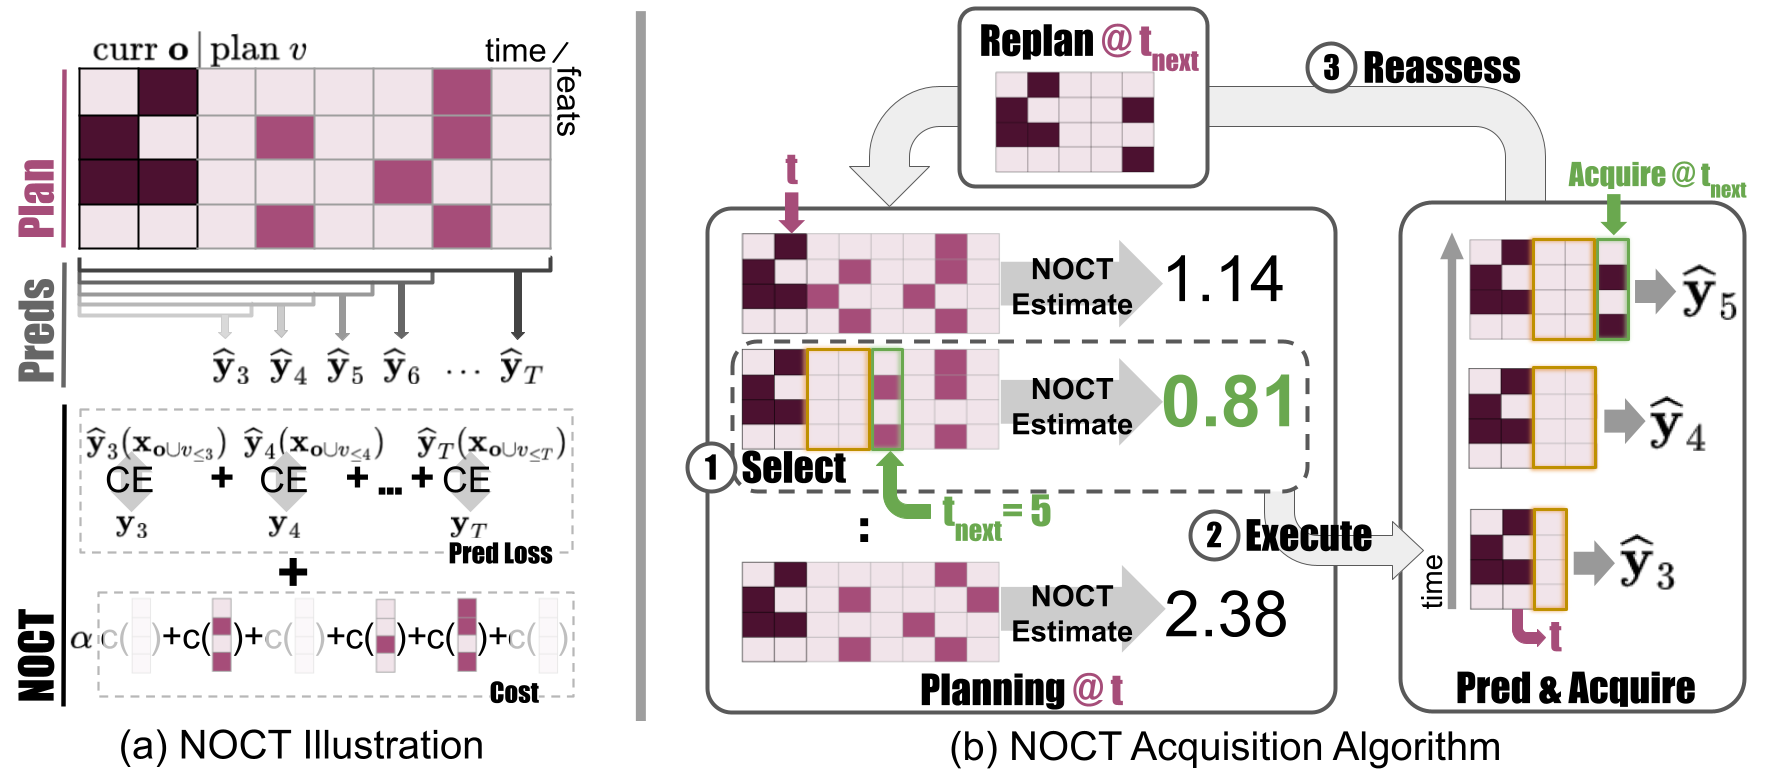
\includegraphics[trim={0cm 0cm 0cm 0cm}, clip, width=0.825\textwidth]{figures/NOCTA_highlevel.png}
    \caption{Overview of \texttt{\OurMethod}. \textbf{(a) NOCT evaluation of plan.}  Given partially observed state $(x_o, o, t)$, a candidate plan $v \subseteq \mathcal{V}_{>t}$ (a feature$\times$time matrix) is evaluated by the tradeoff of (i) the expected accumulated predictive cross-entropy (CE) loss for future acquisitions from $t+1$ to $L$ and (ii) the acquisition cost of selected future acquisitions (i.e., $\alpha \sum_{(m, t') \in v} c^m$). Under plan $v$, the prediction at future time $k$ only uses acquisitions up to time $k$ (i.e., $\hat{y}_{k}(x_{o\cup v_{\le k}})$).
    \textbf{(b) Acquisition algorithm.} At state $(x_o, o, t)$, the \texttt{NOCTA} algorithm evaluates candidate plans $v \subseteq \mathcal{V}_{>t}$ with a NOCT estimator. (1) We \emph{select} the best plan, $\hat{u}$, according to the NOCT estimates. (2) We \emph{execute} the selected plan up to its next acquisition (i.e., $t_{\text{next}}\equiv\min{t':(m,t')\in \hat{u}}$) by acquiring $a_{t_{\text{next}}} \equiv \{(m,t_{\text{next}})\in \hat{u}\}$. Predictions are made at every timepoint; e.g., as illustrated, with $t=2$ and $t_{\text{next}}=5$, \texttt{\OurMethod} predicts at $t=3, 4$ using current information (i.e., $\hat{y}_{3}(x_o), \hat{y}_{4}(x_o))$ and predicts at $t_{\text{next}}=5$ using newly observed features (i.e., $\hat{y}_{5}(x_{o\cup a_{t_{\text{next}}}})$). (3) We \emph{reassess} with $x_o \equiv x_{o\cup a_{t_{\text{next}}}}$ and $t \equiv t_\text{next}$, repeating until the selected plan is empty ($\hat{u}=\varnothing$) or when we reach the final time step ($t= L$). 
    }
    \label{fig:noct}
\end{figure*}

\subsection{NOCT Acquisition (\OurMethod)}

At time $t$, one may use NOCT (Eq.~(\ref{eq:obj})) to indicate the best anticipated future acquisition plan given the current information, $u\bigl(x_o, o\bigr)$:
\begin{equation}
u\bigl({x}_{o}, o\bigr)  \equiv  
\underset{v \subseteq  \mathcal{V}_{>t}}{\arg\!\min}\, \mathrm{NOCT}({x}_{o}, o, v);
\label{eq:nocta}
\end{equation}
i.e., plan according to the anticipated cost tradeoff of obtaining future features for future prediction targets. In fact, we can show that the \texttt{NOCTA} criterion in Eq.~(\ref{eq:nocta}) is a principled proxy value for partially acquired states:
\begin{theorem}
\label{thm:lowerbound}
(Informal) $-\mathrm{NOCT}$ lower bounds the value of the optimal longitudinal AFA MDP policy
\end{theorem}
% \textbf{Theorem 3.1.} \emph{(Informal) The NOCT objective \todo{Dzung: Changed to NOCT} lower bounds the value of the optimal longitudinal AFA MDP policy}.

In other words, acquiring by following the plan selected in Eq.~(\ref{eq:nocta}) serves as an approximation to the optimal longitudinal AFA MDP policy (full proof in Appx.~\ref{appendex:theorem}).




\textbf{Acquisition Algorithm}\quad When Eq.~(\ref{eq:nocta}) returns $u\bigl(x_o, o\bigr) = \varnothing$, it indicates that the potential loss improvement does not justify the cost of acquiring further future features, so we stop acquiring and predict for all subsequent time points using the currently observed features $x_o$. Otherwise, if a non-empty plan $u\bigl(x_o, o\bigr) = v \subseteq \mathcal{V}_{>t}$ is selected, it indicates that, given $x_o$, the set $u\bigl(x_o, o\bigr)$ yields the best trade-off for future predictions. Carrying out the selected plan $u\bigl(x_o, o\bigr)$, implies that the next acquisition occurs at $t_{\text{next} } \equiv \min\{\,t'\mid(m,t')\in u(x_o,o)\}$, the earliest timepoint in the plan. This implies that all the predictions until $t_{\text{next} }$ are to be done with the current information, $\hat{y}_{t+1}({x}_{o}), \ldots, \hat{y}_{t_{\text{next}}-1}({x}_{o})$, and the prediction at $t_{\text{next}}$ includes the planned features at $t_{\text{next}}$, $a_{t_{\text{next}}} \equiv \{(m,t_{\text{next}})\mid(m,t_{\text{next}})\in u(x_o,o)\}$, $\hat{y}_{t_{\text{next}}}({x}_{o \cup a_{t_{\text{next}}}})$. We may similarly continue with acquisitions in $u\bigl(x_o, o\bigr)$ for timepoints after $t_{\text{next}}$. However, a more dynamic strategy is to incorporate the newly acquired feature values to reassess (update) the best anticipated plan. That is, compute $u\bigl({x}_{o \cup a_{t_{\text{next}}}}, o \cup a_{t_{\text{next}}}\bigr)$ using $\mathcal{V}_{t_{\text{next}}}$, for further acquisitions after $t_{\text{next}}$ (see Fig.~\ref{fig:noct}(b)). 



% \textbf{Proposition 3.2.} \emph{(Informal) Replanning after each acquisition is never worse (in $\mathrm{NOCT}$ value) than committing to the original plan’s remainder (full proof in Appx. \ref{appendex:proposition1}).}
\begin{proposition}
\label{prop:replanning}
(Informal) Replanning after each acquisition is never worse (in terms of the $\mathrm{NOCT}$ objective) than committing to the original plan’s remainder (full proof in Appx.~\ref{appendex:proposition1}).
\end{proposition}


Note that $u\bigl({x}_{o \cup a_{t_{\text{next}}}}, o \cup a_{t_{\text{next}}}\bigr)$ is a dominating strategy to simply proceeding with $u\bigl(x_o, o\bigr)$ since: 1) it incorporates additional information, which provides more context (using values in $a_{t_{\text{next}}}$) for the anticipated utility of further acquisitions; 2) the search for $u\bigl({x}_{o \cup a_{t_{\text{next}}}}, o \cup a_{t_{\text{next}}}\bigr)$ includes the original plan for further acquisition from $u\bigl(x_o, o\bigr)$, so it may stick to the previous plan if it is still anticipated to be optimal in light of new values. Intuitively, this dynamic strategy avoids a stubborn approach that does not update its acquisition plans in light of additional information. The acquisition process of \texttt{\OurMethod} is detailed in Alg.~\ref{alg:nocta}.

\begin{algorithm}[htp]
    \footnotesize
  \caption{\texttt{\OurMethod} \label{alg:nocta}}
  \begin{algorithmic}[1]
    \Require Number of features $M$, number of time steps $L$, cost for feature $m$ as $c^m$, estimator $\hat y_{k}$.

    \State Initialize: \texttt{predictions} $\gets [\,]$; \texttt{terminate} $\gets$ \texttt{false}; $t \gets 0$; $o \gets \varnothing$
    
    % \State Initialize \texttt{terminate} $\gets$ \texttt{false}
    % \State Initialize $t \gets 1$
    \While{not \texttt{terminate}}
    \State $\mathcal{V}_{>t} \! \gets\!  \{(m,t') \! \mid \! m\in\{1,\ldots,M\},\,t'\in\{t+1,\ldots,L\}\}$
      \State $\hat u(x_o,o)\approx
    \underset{v \subseteq  \mathcal{V}_{>t}} {\arg\!\min}\,\mathrm{NOCT}(x_o, o, v)$ \Comment{Approx.}
      \If{$\hat u(x_o,o)=\varnothing$}
        \State $t_{\text{next} }\gets L$; \texttt{terminate} $\gets$ 
        \texttt{true}
      \Else
        \State $t_{\text{next}}\gets\min\{\,t'\mid(m,t')\in\hat u(x_o,o)\}$
        \State $o\gets o\cup\{(m,t_{\text{next}})\mid(m,t_{\text{next}})\in\hat u(x_o,o)\}$
      \EndIf
        \For{$t' = t+1,\dots,t_{\text{next}}$}
          \State append $\hat{y} _{t'}\bigl(x_{o_{1:t'}}\bigr)$ to \texttt{predictions}
        \EndFor
        \State $t \gets t_{\text{next}}$
%
    \EndWhile
    \State \Return \texttt{predictions}
  \end{algorithmic}
\end{algorithm}

Note that NOCT (Eq.~(\ref{eq:obj})) is not directly tractable at inference time, since it requires knowledge of the ground-truth conditionals $y_{t+1:L}, x_v \mid {x}_{o}$; thus, we proceed with estimate of NOCT and $u(x_o, o)$, which we develop below. 
% \textbf{Proposition 2} \emph{(Informal) If $\widehat{\mathrm{NOCT}}$ estimates $\mathrm{NOCT}$ within $\varepsilon$ error at each replanning round, then the resulting policy is at most $O(s\varepsilon)$ worse than oracle-\texttt{\OurMethod}, where $s$ is the maximum number of remaining acquisition rounds (proof in Appx. \ref{appendex:regret}).}

% In other words, this implies that a small error in $\widehat{\mathrm{NOCT}}$ cannot cause a large degradation in the overall sequential decision plan, and the bound degrades only linearly with the number of acquisition rounds $s$.

% are acquired, the model predicts for the subsequent time points until the next scheduled acquisitions. 
% This non-greedy policy for \texttt{\OurMethod} 
% %is \emph{simpler to estimate than a full MDP solution, yet still 
% directly balances the tradeoff between acquisition cost and predictive performance. 

%  The acquisition process of \texttt{\OurMethod} is detailed in Algorithm~\ref{alg:nocta}. Intuitively, \texttt{\OurMethod} mirrors the clinical workflow: order tests, read results, and reassess. When \texttt{\OurMethod} selects the acquisition plan $\hat u(x_o,o)$, we do not commit to the entire sequence. Instead, we only execute the acquisition scheduled at the immediate next time point $t_{\text{next}}$, update the observed features $(x_o,o)$, and replan the acquisition schedule. Note that the model can also continue on with its original plan if it still believes those remaining acquisitions are optimal in light of the new acquired information in $t_\text{next}$. This iterative design reflects the principle that as new observed features alter our belief about the labels, it should also update our estimate of the utility of yet-to-be-acquired information.




 % However, evaluating this objective is intractable as in practice we do not have access to the true expectation of labels and unacquired values for the test samples, $\mathbb{E}_{y_{t+1:L}, x_v \mid {x}_{o}}$ in Eq. (\ref{eq:obj}). We therefore develop two ways to estimate $u\bigl({x}_{o}, o\bigr)$: a non-parametric method that uses nearest neighbors on learned embedding space (Sec. \ref{subsec:nonparam}) and a parametric method that directly predicts the accuracy-cost tradeoff (Sec. \ref{subsec:param}). 

% Following \cite{valancius2023acquisition}, one may connect our \texttt{\OurMethod} acquisition objective (Eq. (\ref{alg:nocta})) to the full RL optimization via a lower bound.
% % In other words, the optimal longitudinal AFA MDP policy is guaranteed to perform no worse than \texttt{NOCTA}. A proof of this result can be found in Appendix \ref{appendex:theorem}.
% In other words, acquiring according to the \texttt{NOCTA} objective (Eq. (\ref{eq:obj})) serves as an approximation to the optimum longitudinal AFA MDP. Additional details can be found in Appendix \ref{appendex:theorem}.

% Following \cite{valancius2023acquisition}, one may connect our \texttt{\OurMethod} acquisition objective (Eq. (\ref{alg:nocta})) to the full RL optimization via a lower bound:

% To connect our \texttt{\OurMethod} acquisition objective (Eq. (\ref{alg:nocta})) to the full RL optimization, we cast both problems to maximization and have the following guarantee:

% \textbf{Theorem 1.} \emph{The value of the optimal longitudinal AFA MDP policy is lower bounded by \texttt{\OurMethod}}.

% % In other words, the optimal longitudinal AFA MDP policy is guaranteed to perform no worse than \texttt{NOCTA}. A proof of this result can be found in Appendix \ref{appendex:theorem}.
% In other words, acquiring according to the \texttt{NOCTA} objective (Eq. (\ref{eq:obj})) serves as an approximation to the optimum longitudinal AFA MDP. A proof of this result can be found in Appendix \ref{appendex:theorem}.

% \begin{algorithm}[tb]
%   \caption{\texttt{\OurMethod}: Non‑Greedy Optimal Cost–Tradeoff Acquisition}
%   \label{alg:nocta}
%   \begin{algorithmic}[1]
%     \Require Observed features $o$ (possibly $o=\varnothing$), instance values $x_{o}$, \\
%              \quad\;\;number of features $M$, number of timesteps $L$, \\
%              \quad\;\;costs $c^{a}$ for each feature $a$, trade‑off $\alpha>0$, estimator $f_{k}$
%     \Ensure A sequence of intermediate predictions \texttt{predictions}
%     \State \textbf{initialize} \texttt{terminate} $\gets$ \texttt{false}
%     \State \textbf{initialize} \texttt{predictions} $\gets [\,]$
%     \State \textbf{initialize} $t \gets 1$
%     \While{$t \le L$ \textbf{and} not \texttt{terminate}}
%       \State $V \gets \{(m,t') \mid m\in\{1,\dots,M\},\,t'\in\{t,\dots,L\}\}\setminus o$
%       \State $\hat u \;\gets\;\displaystyle
%         \underset{v\subseteq V}{\arg\min}\Bigl[
%           \E_{y_{t:L},x_v\mid x_o}\,\ell(x_o\cup x_v,y,t)
%           \;+\;\alpha\sum_{a\in v}c^a
%         \Bigr]$
%       \If{$\hat u = \varnothing$}
%         \State \texttt{terminate} $\gets$ \texttt{true}
%       \Else
%         \State $t_{\min}\gets \min\{t'\mid(m,t')\in\hat u\}$
%         \State $o\gets o\;\cup\;\{(m,t_{\min})\mid(m,t_{\min})\in\hat u\}$
%         \For{$i = t,\dots,\min(t_{\min},L)$}
%           \State $\hat y_i \gets f_{k}\bigl(x_{o,1:i}\bigr)$
%           \State append $\hat y_i$ to \texttt{predictions}
%         \EndFor
%         \State $t \gets t_{\min}$
%       \EndIf
%     \EndWhile
%     \State \Return \texttt{predictions}
%   \end{algorithmic}


% \subsection{\texttt{NOCT-Contrastive}}
\subsection{\texttt{NOCT-Contrastive}}
\label{subsec:nonparam}

In this subsection, we introduce \texttt{NOCT-Contrastive}, an embedding-based estimator that enables estimating $\mathrm{NOCT}(x_o,o,v)$ (and therefore $u({x}_{o}, o)$) from partial observations. We train the embedding space with a contrastive loss that embeds instances according to the utility of future acquisitions.

\textbf{Plug-in NOCT}\quad For \emph{training instances}, $(x_i, y_i) \in \mathcal{D}$, the simplest estimate of $\mathrm{NOCT}\bigl({x}_{i,o}, o, v\bigr)$ (Eq.~(\ref{eq:obj})) is a plug-in sample approach:
\begin{equation}
    \scalebox{0.9}{$\displaystyle
        \widehat{\mathrm{NOCT}}_{pl}\bigl({x}_{i,o}, o, v\bigr) =\ell (x_{i,o} \cup x_{i,v}, y_i, t) + \alpha \!\!\! \sum_{(m, t') \in v} \!\!\! c^m.
    $}
    \label{eq:plugobj}
\end{equation}
Note that for a held-out instance, Eq.~(\ref{eq:plugobj}) is not directly computable (it requires future features $x_{i,v}$); we develop inference-time estimators later in this section. For a training instance, we may determine what features are useful when starting from $o$ at time $t$ by ranking candidate future plans $v \subseteq V_{>t}$ using the plug-in objective $\widehat{\mathrm{NOCT}}_{\mathrm{pl}}(x_{i,o},o,v)$ and taking the top-$r$ plans $\hat{v}_{i,o}^{(1)}, \ldots, \hat{v}_{i,o}^{(r)}$ with the smallest values. These top plans induce a future-candidate distribution, $\zeta_{i,o}$, \emph{over future acquisitions} $(m, t')\in V_{>t}$ (and termination $\varnothing$), where $\zeta_{i,o}(m,t')$ is given by a normalized count of how often $(m,t')$ appears in $\hat{v}_{i,o}^{(1)}, \ldots, \hat{v}_{i,o}^{(r)}$. Intuitively, $\zeta_{i,o}$ summarizes which \emph{future} measurements are consistently suggested by the best plans, and we use it in our contrastive loss. The formal $\zeta_{i,o}$ construction in Appx.~\ref{appendex:future_dist}. 

% These top plans induce a future-candidate distribution, $\zeta_{i,o}$, over future acquisitions $(m, t')\in \mathcal{V}_{>t}$  (by a normalized count of occurrences in $\hat{v}_{i,o}^{(1)}, \ldots, \hat{v}_{i,o}^{(r)}$) that we propose to use in a contrastive loss. The formal construction is provided in Appx. ~\ref{appendex:future_dist}
%We construct $\zeta_{i,o}$ as follow: we assign higher weight to plans with lower $\widehat{\mathrm{NOCT}}_{pl}$, count how often each acquisition $(m,t')$ appears among the weighted top-$r$ plans, and normalize the resulting nonnegative scores to sum to $1$. 
% Thus, $\zeta_{i,o}$ is a categorical distribution supported on $\mathcal V_{>t}$ (and $\varnothing$ for termination for empty set $\hat{v}_{i,o}$), where $\zeta_{i,o}(m,t')$ is larger when $(m,t')$ is repeatedly selected by many high-quality plans. Intuitively, $\zeta_{i,o}$ summarizes which future acquisitions are repeatedly favored under the accuracy-cost objective (Eq. (\ref{eq:plugobj})) from the current observed info $x_o$. 

\textbf{Contrastive Learning}\quad We propose to learn an embedding network that maps partially observed features into an embedding space where distances capture the similarity of their acquisition characteristics. Formally, we learn an embedding network $g_\phi(x_{i,o}) \in \mathbb{R}^E$ such that two instances $x_{i,o}$ and $x_{j,o}$ are mapped to nearby points in $\mathbb{R}^E$ if the additional (future) acquisitions available to them are expected to influence their accuracy-cost tradeoff in a similar manner. Conversely, instances with divergent accuracy-cost tradeoff are pushed away in $\mathbb{R}^E$. 

To achieve this, we define a similarity score between instances based on their future-candidate distributions $\zeta_{i, o}$ and $\zeta_{j, o}$, using the exponential of their negative Jensen-Shannon ($\mathrm{JS}$) divergence:
\begin{equation}
      \texttt{sim}_{ij}
    = \exp\!\bigl(-\beta\,\mathrm{JS}(\zeta_{i, o}, \zeta_{j, o})\bigr),
    \label{eq:js}
\end{equation}
where $\beta > 0$ controls how strongly divergence affects similarity. Letting $\delta_{ij} = \bigl\lVert g_\phi \bigl(x_{i,o}\bigr) - g_\phi\bigl(x_{j, o}\bigr)\bigr\rVert^2$ be the embedding distance, we minimize a contrastive loss \citep{chopra2005learning}:
\begin{equation}
\label{eq:ebmedding}
    \scalebox{0.87}{$\displaystyle
    \mathcal{L}_{\mathrm{emb}} = \frac{1}{2} \Bigl(\texttt{sim}_{ij} \cdot \delta_{ij} + 
    (1 - \texttt{sim}_{ij}) \cdot \max \bigl(0,\,\gamma - \delta_{ij}\bigr)^2\Bigr)$},
\end{equation} 
where $\gamma > 0$ is the margin parameter. Minimizing $\mathcal{L}_{\mathrm{emb}}$ encourages $g_\phi$ to create an embedding space where distance reflects the similarity of future-candidate distributions. 

\textbf{\texttt{NOCT-Contrastive}}\quad For held-out instances (at inference time), the plug-in estimate $\widehat{\mathrm{NOCT}}_{pl}$ in Eq.~(\ref{eq:plugobj}) is unavailable because future measurements and labels are unknown. Instead, we approximate $\mathrm{NOCT}(x_o,o,v)$ by aggregating plug-in values from a small retrieved set of training trajectories selected by the learned embedding:
% Instead, we propose to utilize an instance based approach using the proposed embeddings (Eq.~\ref{eq:ebmedding}):
\begin{equation}
\scalebox{0.93}{$\displaystyle \widehat{\mathrm{NOCT}}\bigl({x}_{o}, o, v\bigr)\approx \frac{1}{|\mathcal{I}(x_o)|}\sum_{i \in \mathcal{I}(x_o)} \widehat{\mathrm{NOCT}}_{pl}\bigl({x}_{i,o}, o, v\bigr),$} 
\label{eq:noctanp}
\end{equation}
where $\mathcal{I}(x_o)$ contains the closest training instances induced by $g_\phi$: $d(x_o, x_{i,o}) = \Vert g_\phi{(x_o)} - g_\phi{(x_{i,o})} \Vert_{2}$ (e.g., by distance thresholding or by selecting the top-$K$ most similar instances). Note that since $g_\phi(x_{o})$ embeds instances according to the utility of future acquisition, estimating $\mathrm{NOCT}\bigl({x}_{o}, o, v\bigr)$ in terms of $\widehat{\mathrm{NOCT}}_{pl}\bigl({x}_{i,o}, o, v\bigr)$ for $i\in \mathcal{I}(x_o)$ is a sound, intuitive strategy. Note further that the size of the embedding space is a controllable hyperparameter, enabling efficiency at small dimensionalities. We call this estimator \texttt{NOCT-Contrastive}.

$\widehat{\mathrm{NOCT}}\bigl({x}_{o}, o, v\bigr)$ enables us to estimate $\hat{u}(x_o, o)$ in Alg.~\ref{alg:nocta}, to plan acquisitions at inference time. In practice, instead of an exhaustive search over  $v\subseteq \mathcal{V}_{>t}$, one may consider a distributionally sampled (e.g., uniform random or feature-importance guided) set of candidate plans. 
%of  provides a fast approximation to $\arg\min_{v\subseteq \mathcal{V}^{>t}}\widehat{\mathrm{NOCT}}(x_o,o,v)$ and performs well in our experiments. 
More sophisticated discrete optimizers could be substituted if desired, but typically introduce additional overhead \citep{parker2014discrete, rajeev1992discrete}.

\subsection{\texttt{NOCT-Amortized}}
\label{subsec:param}

%Section~\ref{subsec:nonparam} presented an \emph{instance-based} estimator of $\mathrm{NOCT}(x_o,o,v)$ that averages utilities over training instances in a learned embedding space. 
We now develop \texttt{NOCT-Amortized}, a complementary
approach that amortizes inference and predicts the NOCT value for candidate acquisition plans using a neural network. %We coin this estimator as \texttt{NOCT-Amortized}. 


\textbf{Neural NOCT estimator}\quad We learn an estimator $f_\theta$ that predicts the NOCT value of a candidate plan from \emph{the partial information} $x_o$. Since future features $x_v$ are unknown at inference time, $f_\theta$ is conditioned on
the partial observations $x_o$, a representation of the candidate plan $v$ (e.g., a binary mask over feature-time pairs in $V_{>t}$),
and the current time $t$:
\begin{equation}
f_\theta(x_o, v, t) \;\approx\; \mathrm{NOCT}(x_o,o,v).
\label{eq:noct_direct_pred}
\end{equation}
At inference time, we substitute Eq.~\eqref{eq:noct_direct_pred} into  Alg.~\ref{alg:nocta} and obtain the future candidate plan:
\begin{equation}
\hat u(x_o,o) \;\in\; \arg\min_{v \subseteq V_{>t}} f_\theta(x_o, v, t).
\end{equation}
\paragraph{Training Objective}
During training, we can compute the plug-in target $\widehat{\mathrm{NOCT}}_{pl}(x_o,o,v)$ in Eq.~\eqref{eq:plugobj} because the
ground-truth future values for $x_v$ are available in $\mathcal{D}$. We train $f_\theta$ by minimizing the mean squared error objective:
\begin{align} 
\mathcal{L}_{\mathrm{amort}} ~=~  \big( f_\theta(x_{o}, v, t) - \widehat{\mathrm{NOCT}}_{pl}(x_{o}, o, v) \big)^2. 
\label{eq:value_mse} 
\end{align}
\paragraph{Joint Fine-tuning with the Predictor} To reduce the mismatch between (i) the partially observed inputs used by the predictor $\hat y$ and (ii) the inputs scored by $f_\theta$ during planning, we jointly fine-tune $f_\theta$ and $\hat y$ with
\begin{align}
\mathcal{L}_{\mathrm{joint}}
~=~
\frac{1}{L}\sum_{k=1}^{L} \mathrm{CE}\!\left(\hat y_k(x_{o_{1:k}}), y_k\right)
~+~ \lambda\,\mathcal{L}_{\mathrm{amort}},
\label{eq:direct_joint}
\end{align}
where $\lambda$ trades off predictive accuracy and utility estimation. 

% \todo{Phrase search of plan subsampling as a benefit: many methods could be applied, even simple appraoch works.}

% \todo{JO: what is the major idea??} %In non-parametric setup, once we decide the next desired timepoint, we simultaneously acquire all desired features (for more details, please refer to Alg. \ref{alg:lafanp}).



% Note that applying Eq.~\eqref{eq:prob} to specific training data $(x_i, y_i) \in \mathcal{D}$ having observed feature $o$ will yield its future-candidate distribution $p(\cdot \mid x_{i,o})$.


% two samples $x_i$ and $x_j$ with the same observed feature o is computed as $d(x_{i,o}, x_{j,o}) = \Vert g_\phi (x_{i,o}) - g_\phi(x_{j,o}) \Vert_{2}$.

% We train an embedding network $g_\phi: x_o \mapsto \mathbb{R}^E$ so that two partial observations $x_{i, o}$ and $x_{j,o}$  with similar future distributions $p(\cdot \mid x_{i,o})$ and $p(\cdot \mid x_{j,o})$ lie close in the embedding space, and those with dissimilar distributions lie farther apart. To quantify similarity, we use the exponential of the negative Jensen-Shannon (JS) divergence between these two distributions:
% \begin{equation}
%       \texttt{sim}_{ij}
%     = \exp\!\bigl(-\beta\,\mathrm{JS}(p(\cdot \mid x_{i,o}),\,p(\cdot \mid x_{j,o}))\bigr),
% \end{equation}
% % \end{equation}
% and $\beta>0$ controls how strongly divergence affects similarity. Let 
% \begin{equation}
%       \delta_{ij} = \bigl\lVert g_\phi \bigl(x_{i,o}\bigr) - g_\phi\bigl(x_{j, o}\bigr)\bigr\rVert^2
% \end{equation}
% be the squared distance between embeddings of two partial observations $\bigl(x_{i,o}, x_{j,o}\bigr)$. The embedding loss $\mathcal{L}_{\mathrm{emb}}$ is then defined as a contrastive-type loss \citep{chopra2005learning}:
% {\small
% \begin{equation}
% \label{eq:ebmedding}
%     \mathcal{L}_{\mathrm{emb}} = \frac{1}{2} \Bigl(\texttt{sim}_{ij} \cdot \delta_{ij} + 
%     (1 - \texttt{sim}_{ij}) \cdot \max \bigl(0,\,\gamma - \delta_{ij}\bigr)^2\Bigr),
% \end{equation}
% }where $\gamma>0$ is the margin parameter. Minimizing $\mathcal{L}_{\mathrm{emb}}$ encourages pairs of samples whose future distributions are similar (low JS divergence) to have low Euclidean distance in the embedding space, while pairs with dissimilar distributions (high JS divergence) are pushed apart by a margin. Finally, the distance for two samples $x_i$ and $x_j$ with the same observed feature $o$ is computed as $d\bigl(g_\phi (x_{i,o}), g_\phi(x_{j,o})\bigr)$.


% \subsection{\texttt{\OurMethod-Direct}: Direct Neural Network Estimate}
% \label{subsec:param}

% Section~\ref{sec:noct_est} presented an \emph{instance-based} estimator of $\mathrm{NOCT}(x_o,o,v)$ that averages
% trajectory-level utilities over nearest neighbors in a learned embedding space. We now describe a complementary
% approach that \emph{directly} predicts the NOCT objective for a candidate acquisition plan, avoiding neighbor search at
% test time.

% \todo{Rephrase to be consistent with above. E.g. "instance-based" and use NOCT equations}
% Above, we proposed a non-parametric, neighbor-based approach to estimate our generalized \texttt{\OurMethod} cost objective Eq.~(\ref{eq:obj}). We also develop a direct parametric approach, which estimates the cost objective using a network. We expound on our parametric approach, coined \texttt{\OurMethod-P}, below. 

% \textbf{Estimating $u\bigl({x}_{o}, o\bigr)$.} In order to estimate $u(x_o, o)$ in Eq.~(\ref{eq:obj}) parametrically, we attempt to calculate the utility for all potential subsets $v \subseteq \mathcal{V}$ at current time $t$:
% \begin{equation}
% I_v(x_o, o, t) = \ell (x_o \cup x_v, y, t) + \alpha \!\!\!\! \sum_{(m, t') \in v} \!\!\!\! c^m.
% \label{eq:I}
% \end{equation}
% Since we have access to data during training, this value can be directly calculated for all subsets $v$ for training instances $(x_i, y_i)$. However, this is not the case during evaluation time when $x_v$ becomes unknown. Therefore, we estimate $I_v(x_o, o, t)$ through a value network, which we describe below. 

% \textbf{Value Network.}\quad The value network $f_{\theta}$ predict the utility $I_v(x_o, o, t)$ for all potential subsets. Since future features $x_v$ are unknown during evaluation, the network is only conditioned on observed features $x_o$, a candidate mask $v$, and the current time $t$; and its output is denoted as $f_{\theta}(x_o, v, t)$. Since this output estimates the utility of  $I_v(x_o, o, t)$, we optimize through the mean squared error as:
% \begin{equation}
%     \mathcal{L}_{\mathrm{value}} = \mathrm{MSE}\left(f_{\theta}(x_o, v, t), I_{v}(x_o, o, t)\right)\,.
% \end{equation}
    

% % During inference, the values of the potential subset $x_v$ are not available until we decide to acquire them, hence 
% % To avoid distribution shift during evaluation, we match the distribution of observed subsets $o$ during training to what shall be encountered at inference time. That is, at each acquisition step for both training and inference, we choose the next subset based on $u(x_o, o)=\arg\min_{v \subseteq V} f_\theta(x_o, v, t)$.

% Using this value network, we can estimate Eq.~(\ref{eq:obj}) to derive the future acquisition plan $u\bigl({x}_{o}, o)$.

% To minimize the distribution shift between the features evaluated by the value network and those used by the predictor, we jointly optimize the prediction network $\hat{y}_k$ and the value network $f_{\theta}$ over the candidate subset, resulting in the final loss function as:
% \begin{equation}
%     \mathcal{L}_{\mathrm{\OurMethod\text{-}P}} = \frac{1}{L}\sum_{k=1}^{L}{\mathrm{CE}\bigl(\hat{y}_k({x}_{o_{1:k}}), y_{k}\bigr)} + \lambda \cdot \mathcal{L}_{\mathrm{value}} \,,
%     % \mathcal{L}_{\mathrm{\OurMethod\text{-}P}} = \mathcal{L}_{\mathrm{pred}} + \lambda \cdot \mathcal{L}_{\mathrm{value}} \,,
% \end{equation}
% where $\lambda$ balances the tradeoff between minimizing the prediction error (the cross-entropy loss) and accurately estimating the utility of future acquisitions with the value network ($\mathcal{L}_{\mathrm{value}}$).

% % prediction network loss and the value network loss $\mathcal{L}_{\mathrm{value}}$. 

% % We further describe prediction network and its loss function $\mathcal{L}_{\mathrm{pred}}$ in Sec.~\ref{sec:implementation}.
% % where $\lambda$ balances the prediction network loss $\mathcal{L}_{\mathrm{pred}}$ (e.g., cross-entropy) and the value network loss $\mathcal{L}_{\mathrm{value}}$. We further describe prediction network and its loss function $\mathcal{L}_{\mathrm{pred}}$ in Sec.~\ref{sec:implementation}.
\section{Experiments}
\label{sec:experiment}
% \subsection{Experimental Setup} 
\subsection{Datasets}
\textbf{Synthetic}\quad Inspired by \citet{kossen2022active}, we construct a synthetic dataset of $N=8,000$ samples with $L=10$ non-i.i.d. timepoints. Each timepoint contains two features: \textit{digit} and \textit{counter}. Labels are the cumulative sum of the digits, when the counter values are zero. We elaborate below.

% a sequence of \textit{digit} features that are summed at locations where \textit{counter} feature indicates (with a zero value). That is, the output labels are comprised of the cumulative sum of the counter-indicated digits. We expound below.


The \textit{digit} feature is a sequence of uniformly random $L$ integers from $\{0, 1, 2\}$, e.g., $1010220110$. The \textit{counter} feature is created by concatenating countdown sequences that begin with randomly chosen starting values from $\{0, 1, 2\}$ and truncating to a fixed length of $L$. For example, starting values $2$, $1$, $2$, and $1$ yield $210$, $10$, $210$, $10$, and the final counter feature is their concatenation $2101021010$ (of length $L$). Unlike \citet{kossen2022active}, we assign labels at every timestep: 
% $y_t$ is the cumulative sum of the digit values up to time $t$ (inclusive) where the corresponding counter value is $0$, i.e.,
$y_t=\sum_{t'=1}^{t}\mathrm{digit}_{t'}\mathbb{I}\{\mathrm{counter}_{t'}=0\}$; for example, label $0011333444$ in the case of $\genfrac{}{}{0pt}{}{\mathrm{counter:}}{\mathrm{digit:}}  
 \genfrac{}{}{0pt}{}{21\underline{0}1\underline{0}21\underline{0}1\underline{0}}{10\mathbf{1}0\mathbf{2}20\mathbf{1}1\mathbf{0}}$. The policy should begin with acquiring the digit and counter at 
$t=1$, then acquiring the digit at the next anticipated timestep where $\mathrm{counter}=0$, then acquiring the \textit{counter} again to locate the next $\mathrm{counter}=0$ timestep, and repeat. Following \citet{kossen2022active}, we split data into train/val/test ($70\%/15\%/15\%$).

\textbf{ADNI}\quad The Alzheimer's Disease Neuroimaging Initiative (ADNI) dataset\footnote{\url{https://adni.loni.usc.edu}}~\citep{petersen2010alzheimer} is a longitudinal, multi-center, observational study. Patients are categorized into cognitively unimpaired, mild cognitive impairment, and Alzheimer's Disease \citep{o2008staging, o2010validation}. Following~\citet{qin2024risk}, we use $N=1,002$ patients with four biomarkers extracted from PET (FDG and AV45) and MRI (Hippocampus and Entorhinal) across $L=12$ visits, and split the dataset into train/val/test ($64\%/16\%/20\%$). \looseness-1
% Each patient may have a different pattern of missing features or labels, and we only report the results based on those that have a diagnosis label. %Appendix $\ref{sec:cost}$ provides further details.

\textbf{OAI}\quad The Osteoarthritis Initiative (OAI) dataset\footnote{\url{https://nda.nih.gov/oai/}} contains $N=4,796$ patients (left/right knees) monitored up to $96$ months. We use the tabular data from~\citet{chen2024unified} and joint space width, totaling $27$ features per visit across $L=7$ visits. We predict the two clinical scores: Kellgren-Lawrence grade (KLG)~\citep{kellgren1957radiological} (range $0 \sim 4$) and WOMAC pain score~\citep{mcconnell2001western} (range $0 \sim 20$). Following previous works~\citep{chen2024unified,nguyen2024active}, we merge KLG $=0$ and $1$, and define WOMAC $<5$ as no pain and $\geq 5$ as pain, and split the dataset into train/val/test ($50\%/12.5\%/37.5\%$). 

\subsection{Baselines} 
\emph{We \uline{expand the comparisons} performed in recent work} by \citet{qin2024risk} in longitudinal AFA  by comparing to \emph{two other state-of-the-art AFA methods}, {DIME}~\citep{gadgil2023estimating} and {DiFA} \citep{ghosh2023difa}, in addition to the RL method considered by \citet{qin2024risk}.
\begin{figure*}[t] 
  \centering
  % ----- 1st column -------------------------------------------------
  \resizebox{0.85\textwidth}{!}{
  \begin{subfigure}[t]{.24\textwidth}
    \centering
    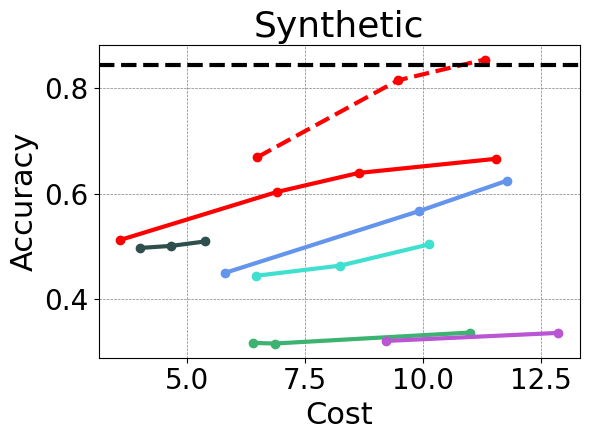
\includegraphics[width=\linewidth]{figures/synthetic.png}
    % \caption{Synthetic}\label{fig:sub1}
  \end{subfigure}
  % ----- 2nd column -------------------------------------------------
  \begin{subfigure}[t]{.24\textwidth}
    \centering
    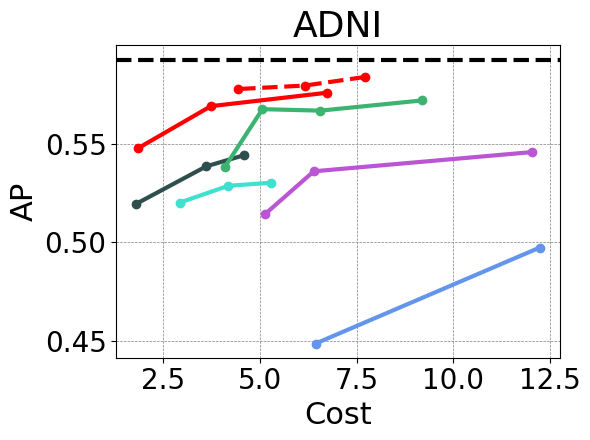
\includegraphics[width=\linewidth]{figures/adni.png}
    % \caption{ADNI}\label{fig:sub2}
  \end{subfigure}
  % ----- 3rd column -------------------------------------------------
  \begin{subfigure}[t]{.24\textwidth}
    \centering
    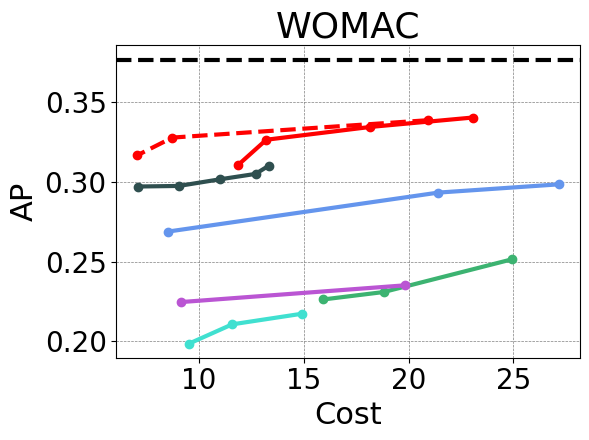
\includegraphics[width=\linewidth]{figures/womac.png}
    % \caption{WOMAC}\label{fig:sub3}
  \end{subfigure}
  % ----- 4th column -------------------------------------------------
  \begin{subfigure}[t]{.24\textwidth}
    \centering
    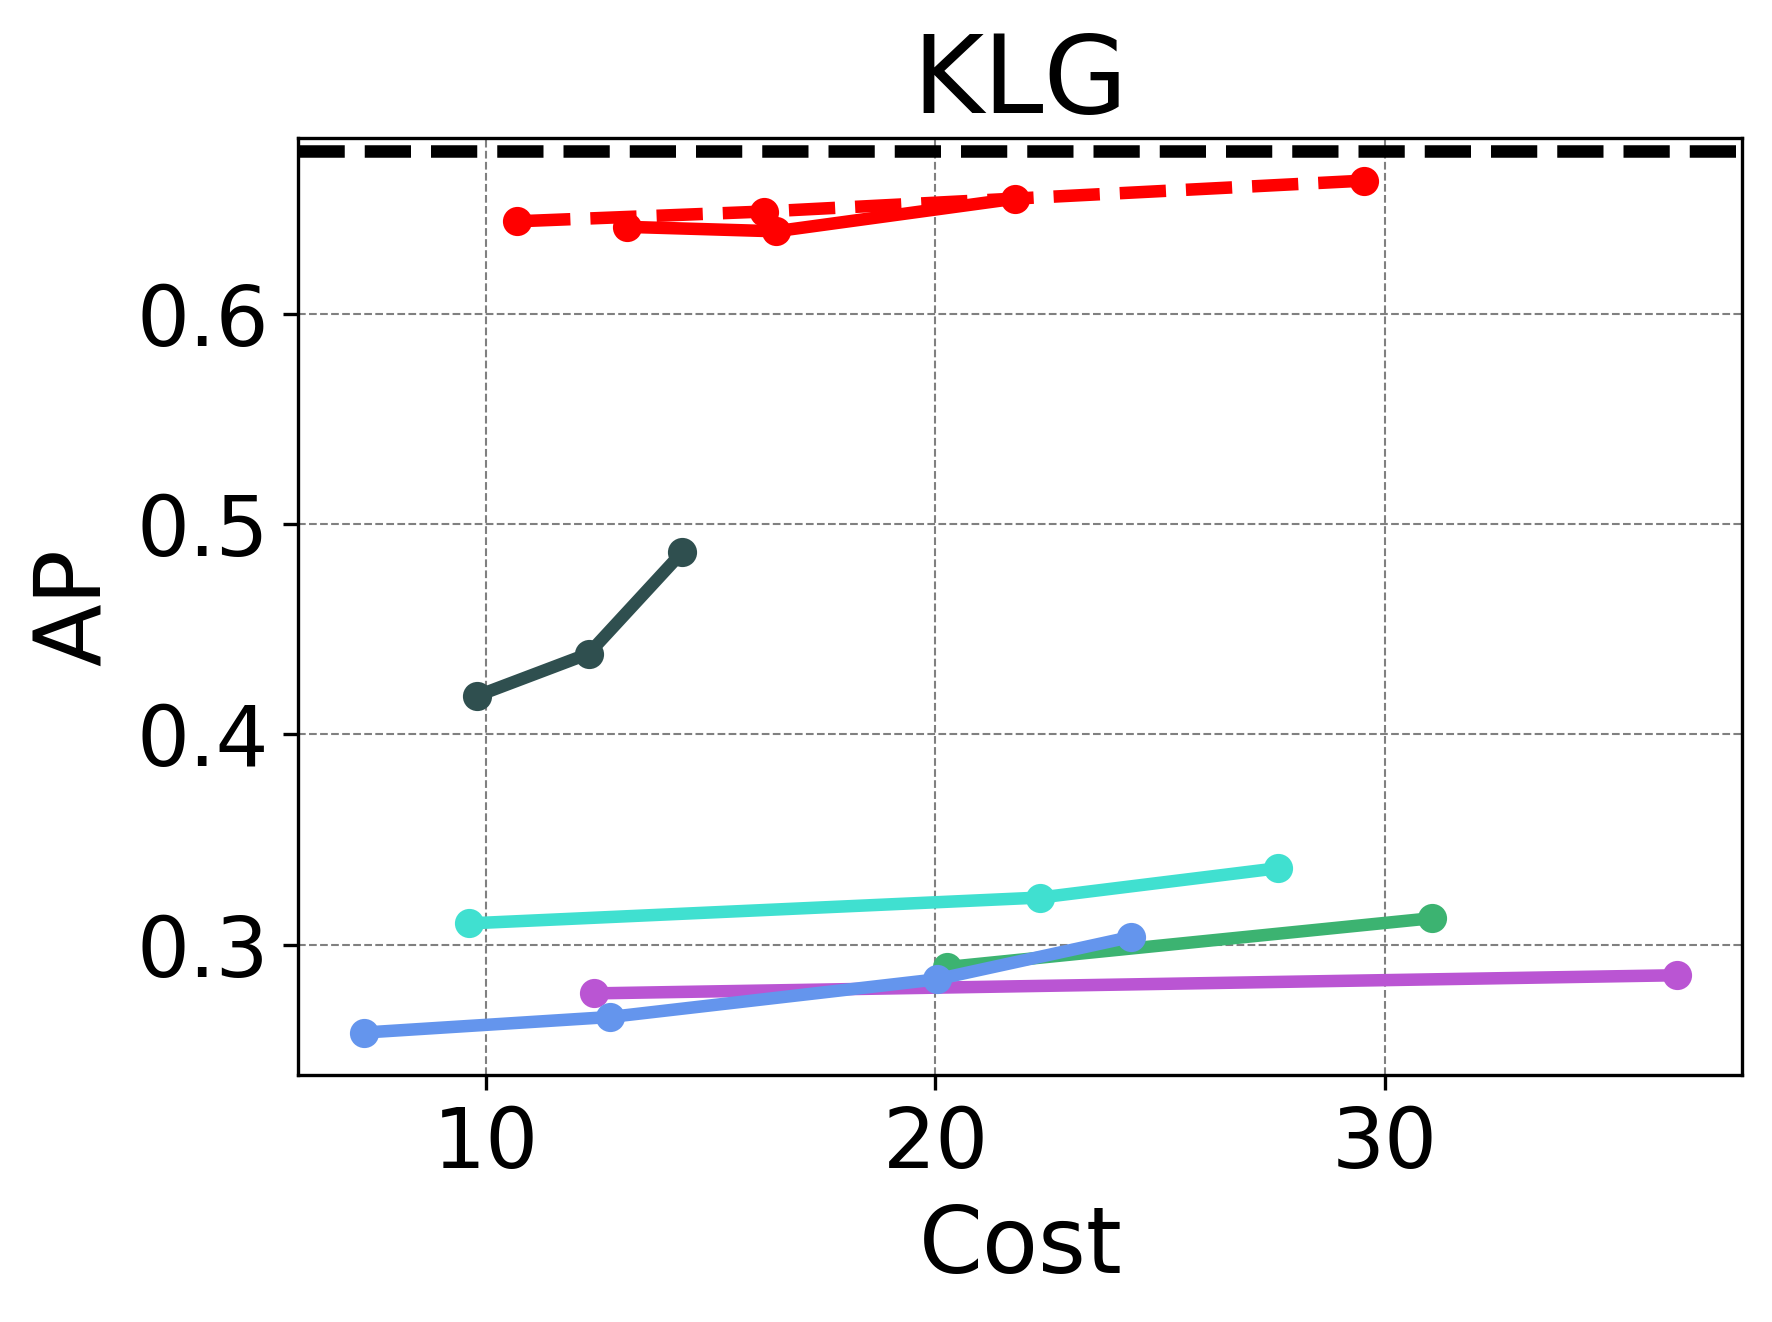
\includegraphics[width=\linewidth]{figures/klg.png}
    % \caption{KLG}\label{fig:sub4}
  \end{subfigure}
  }
  
  % \par\bigskip            % vertical gap between plots and legend
  \vspace{-0.5em}
  \begin{minipage}{\textwidth}
    \centering
    % trim=⟨left bottom right top⟩ clip    — remove surrounding whitespace if needed
    
\includegraphics[width=0.8\textwidth,trim=0 0 0 0,clip]{figures/legend_only.png}
  \end{minipage}
  \vspace{-1em}
  \caption{Performance/cost of  models 
  % on the four benchmarks 
  across various average acquisition costs (budgets). Following~\cite{kossen2022active}, we show accuracy rather than average precision for the synthetic dataset. Our NOCT estimators show the highest accuracy for a given cost. }
  \label{fig:performance}
\end{figure*}

In total, we consider the following baselines: 1) \textbf{ASAC}~\citep{yoon2019asac}: an actor-critic method to jointly train a feature selector and a predictor network; 2) \textbf{RAS}~\citep{qin2024risk}: an RL approach to decide when and which features to capture for longitudinal data where the predicted acquisition times are continuous and not restricted to certain discrete timepoints; 3) \textbf{AS} \citep{qin2024risk}: RAS with a constant acquisition interval; 4) \textbf{DIME}~\citep{gadgil2023estimating}: a greedy method to sequentially select the most informative features; 5) \textbf{DiFA} \citep{ghosh2023difa}: a Gumbel-softmax-based differentiable policy. For each baseline, \emph{we perform a comparable hyperparameter search on the validation set using the authors' original code}, and report test performance under the selected configuration. We also verify reproduction of reported results (e.g., RAS on ADNI); full details are provided in Appx.~\ref{sec:baseline}.


We adapt DIME and DiFA for longitudinal data by restricting acquisitions to either the current or future time points. Note that DIME and DiFA acquire features one at a time, allowing repeated selection within the same time step $t$, while \texttt{\OurMethod} and other baselines simultaneously select all desired features at $t$ before moving to the next time steps. An advantage of DiFA and DIME is that they can acquire more tests now or move to the next visit. \looseness-1


\subsection{Implementation}
\label{sec:implementation}

\textbf{Data Availability and Missingness.} Unlike standard AFA methods that assume fully observed data \citep{rahbar2025survey, shim2018joint, nan2015feature}, our work is general and handles missingness completely at random. This is done by excluding missing features from candidate sets and pretraining the prediction network $\hat{y}_k$, estimator $f_\theta$, and embedding network $g_\phi$ with random input-feature dropout.  


\textbf{Prediction Network Implementation.}  At each time $t$, the prediction network predicts outcomes at future timepoints $\hat{y}_k$, $k \geq t$. We train an MLP that takes all the features observed up to time t, denoted $x_{o_{1:t}}$ \footnote{$x_o$ may contain missingness inherent to the data collection process. Additionally, unobserved features (missing or not acquired) are being masked out during implementation.} and the future time indicator $k$. 
% We then define the prediction network loss as: 
% the prediction network $\hat{y}_k$ uses all features that have been observed up to $t$ (e.g., ${x}_{o_{1:t}}$), combining with future time indicator $k$. That is, we train an MLP that takes $x_{o_{1:t}}$ \footnote{$x_o$ may include missingness due to the inherent noise in data collection. Additionally, unobserved features (missing or not acquired) are being masked out during implementation.} and time indicator $k$ as its input, and apply cross-entropy loss as:
% \begin{equation}
%     \mathcal{L}_{\mathrm{pred}} = \frac{1}{L}\sum_{k=1}^{L}{\mathrm{CE}\bigl(\hat{y}_k({x}_{o_{1:t}}), y_{k}\bigr)}.
% \end{equation}
For predictions at $k > t$, the network must predict without access to any additional features beyond those observed by time $t$ (i.e., $\hat{y}_{k}(x_{o_{1:t}})$ for $k > t$). 


% To mimic the AFA process, the prediction network should be able to predict with any subset of the input features, and hence, we pre-train the prediction network with a random dropout of the input features, whose data are set to $0$. 

\textbf{\texttt{NOCT-Contrastive} Implementation.}\quad
We train the MLP predictor $\hat{y}_k$ and then train the MLP embedding network $g_\phi$. We set $\beta=\gamma=1$, $K=5$, and embedding dimension $E=32$ (Synthetic/ADNI) and $E=64$ (OAI).%, and sample $|\widetilde{\mathcal{V}}|=1000$ subsets.


\textbf{\texttt{NOCT-Amortized} Implementation.}\quad We first train the MLP predictor $\hat{y}_k$, followed by jointly fine-tuning the predictor and the MLP-based NOCT estimator $f_{\theta}$ (Eq.~\ref{eq:value_mse}) using $\lambda=1$.% Both steps use Adam~\citep{kingma2014adam} with a learning rate of $1e-3$ and use $\lambda=1$. We randomly sample $|\widetilde{\mathcal{V}}|=1000$ candidate subsets.

\textbf{Optimizer and Inference}\quad We utilize Adam~\citep{kingma2014adam} with a learning rate of $10^{-3}$. At each inference step, we evaluate a subset of 1,000 plans from the 
candidate space (see Appx. \ref{appendex:sensitivity} for a stability analysis).
% we consider a subset of $1000$   candidate plans

% \textbf{Subset Size $|\mathcal{O}|$.} For experiments, we uniformly sample $1000$ candidate acquisitions to balance effectiveness and overhead. As shown in Appx. $\ref{appendex:sensitivity}$, accuracy stabilizes and returns diminish beyond this cardinality. In practice, we observed uniform sampling is effective and fast, but other discrete optimization methods can be utilized \citep{parker2014discrete, rajeev1992discrete}.

% Following the conventional setup for longitudinal AFA tasks \citep{yoon2019asac, qin2024risk}, we consider each modality as a single feature. 
We report predictive performance results as the mean over five independent runs (standard errors for each run are provided in Appx.~\ref{appendex:results}). Feature costs and further details on the experimental setup can be found in Appx.~\ref{appendex:experiment_setup}. Moreover, Appx.~\ref{appendex:sensitivity} shows a hyperparameter sensitivity analysis, demonstrating that 
\textit{our method remains robust across different settings and can be applied without extensive tuning}.
Upon publication, we will make our code publicly available.


\subsection{Performance-Cost Results}


Fig.~\ref{fig:performance} shows results across different datasets. For each figure, the x-axis represents different average acquisition costs per instance, and the y-axis represents the performance. As the budget increases, more features can be acquired, and prediction performance typically improves. 
We varied hyperparameters to obtain prediction results under different average acquisition costs. Details on the performance-cost tradeoff hyperparameters for each method are in Appx. \ref{appendex:experiment_setup}.
% To obtain points at different average acquisition costs: (1) for RAS, AS, ASAC, and \texttt{\OurMethod‑NP} we sweep the performance-cost tradeoff hyperparameter, (2) DIME and DiFA impose budget limits, and (3) \texttt{\OurMethod‑P} uses both the performance-cost tradeoff hyperparameter and the budget limits. For further details about the trade-off parameter in Appendix \ref{appendex:experiment_setup}.

\textbf{Synthetic Dataset.} Following~\citet{kossen2022active}, we use accuracy for performance on the synthetic dataset. The \texttt{NOCT-Contrastive} estimator outperforms the baselines, followed by the  \texttt{NOCT-Amortized} estimator, suggesting that the baseline methods may not adequately model dependencies between features and necessary acquisitions. 


\textbf{ADNI Dataset.} Following \citet{qin2024risk}, we show the average precision (AP) result for different costs. Both estimator variants of \texttt{\OurMethod} consistently outperform all other baseline methods while using lower overall acquisition cost.
% RAS~\citep{qin2024risk} and DIME~\citep{gadgil2023estimating} also appear to be strong baselines, as they both allows dynamic selection in when and which features to select. AS turned out to be less effective without being able to adapt to the acquisition interval, and ASAC~\citep{yoon2019asac} \todo{add why ASAC not so good}

% \begin{figure*}[!ht]
%   \centering
%   % Left column
%   \begin{minipage}[t]{0.49\textwidth}
%     \centering
%     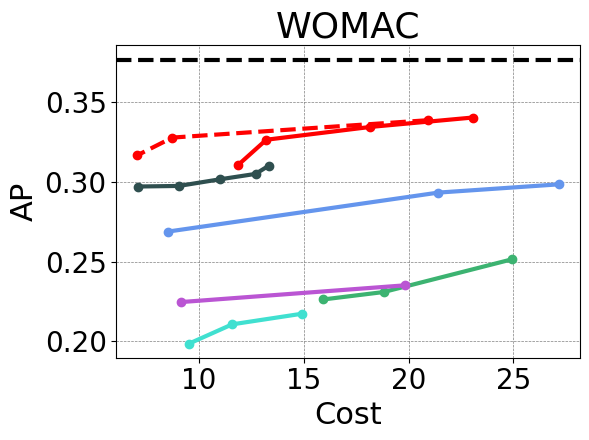
\includegraphics[width=\linewidth]{figures/womac.png}
%     \captionsetup{skip=2pt}
%     \captionof{figure}{AP and ROC vs. average cost on WOMAC prediction}
%     \label{fig:womac}
%   \end{minipage}\hfill
%   \begin{minipage}[t]{0.49\textwidth}
%     \centering
%     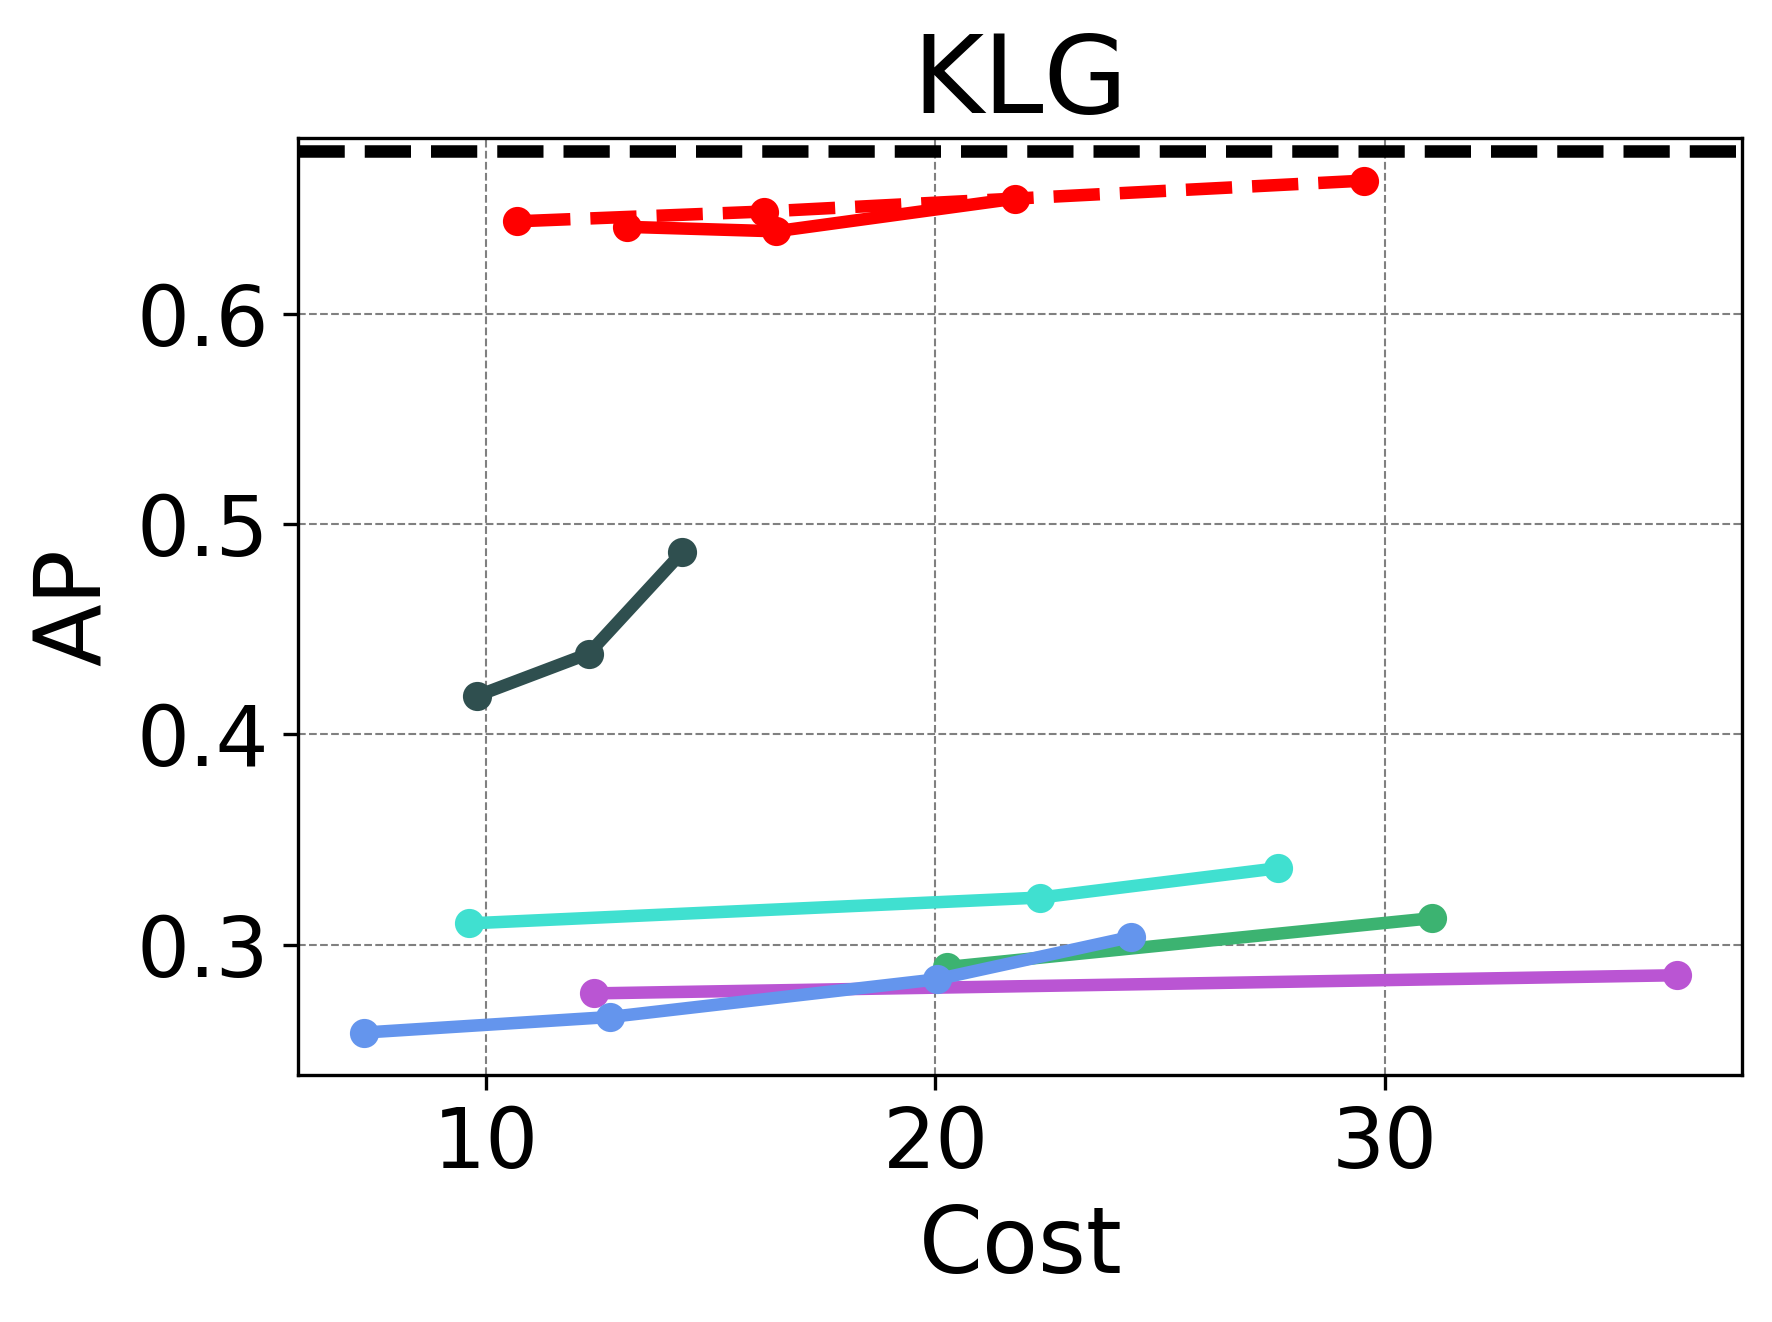
\includegraphics[width=\linewidth]{figures/klg.png}
%     \captionsetup{skip=2pt}
%     \captionof{figure}{AP and ROC vs. averagecost on KLG prediction}
%     \label{fig:klg}
%   \end{minipage}
% \end{figure*}
\textbf{OAI Dataset.} We report AP on KLG and WOMAC prediction (Fig.~\ref{fig:performance}). The \texttt{\OurMethod} again outperforms the baselines, while RL-based approaches (ASAC, AS, and RAS) underperform compared to the greedy approach (DIME), suggesting that RL-based frameworks may struggle with the complexity and noise of longitudinal feature acquisition. 
\begin{table*}[ht]
\captionsetup{skip=2pt}
\caption{Result comparisons of using the feature values, $\hat{y}$ prediction embedding (last hidden layer), and learned representation $g_\phi(\cdot)$ to gather instances for \texttt{NOCT-Contrastive} inference. We report the mean $\pm$ standard errors across five runs.}
\label{tab:embedding}
% \vspace{-0.1in}
\begin{center}
\begin{sc}
\resizebox{1\linewidth}{!}{%
\begin{tabular}{c
                ccc @{\quad}
                ccc @{\quad}
                ccc}
\toprule
\multirow{2}{*}{Method}
  & \multicolumn{3}{c}{ADNI}
  & \multicolumn{3}{c}{WOMAC}
  & \multicolumn{3}{c}{KLG} \\
\cmidrule(lr){2-4} \cmidrule(lr){5-7} \cmidrule(lr){8-10}
 & AP & ROC & cost
 & AP & ROC & cost
 & AP & ROC & cost \\
\midrule
\multirow{2}{*}{\makecell{Feature\\Values}}
 & $0.545\pm0.004$ & $0.727\pm0.002$ & $7.052\pm0.069$
 & $0.315\pm0.003$ & $0.617\pm0.004$ & $9.014\pm2.863$
 & $0.629\pm0.003$ & $0.821\pm0.002$ & $11.024\pm0.011$ \\
 & $0.550\pm0.007$ & $0.732\pm0.008$ & $10.297\pm1.168$
 & $0.331\pm0.013$ & $0.633\pm0.013$ & $17.574\pm0.070$
 & $\mathbf{0.651}\pm\mathbf{0.010}$ & $0.826\pm0.021$ & $17.741\pm0.033$ \\
\midrule
\multirow{2}{*}{\makecell{Prediction\\Embedding}}
 & $0.567\pm0.005$ & $0.744\pm0.004$ & $6.218\pm0.038$
 & $0.290\pm0.005$ & $0.618\pm0.002$ & $6.998\pm0.023$
 & $0.639\pm0.004$ & $\mathbf{0.825}\pm\mathbf{0.002}$ & $13.706\pm0.055$ \\
 & $0.571\pm0.021$ & $0.744\pm0.013$ & $7.866\pm0.068$
 & $0.290\pm0.004$ & $0.618\pm0.002$ & $19.681\pm0.081$
 & $0.648\pm0.001$ & $\mathbf{0.829}\pm\mathbf{0.001}$ & $24.705\pm0.043$ \\
\midrule
\multirow{2}{*}{\makecell{Embedding\\Network}}
 & $\mathbf{0.578}\pm\mathbf{0.004}$ & $\mathbf{0.760}\pm\mathbf{0.003}$ & $4.434\pm0.042$
 & $\mathbf{0.328}\pm\mathbf{0.004}$ & $\mathbf{0.646}\pm\mathbf{0.003}$ & $8.729\pm0.011$
 & $\mathbf{0.644}\pm\mathbf{0.003}$ & $0.822\pm0.001$ & $10.687\pm0.018$ \\
 & $\mathbf{0.584}\pm\mathbf{0.013}$ & $\mathbf{0.760}\pm\mathbf{0.006}$ & $7.727\pm0.094$
 & $\mathbf{0.339}\pm\mathbf{0.008}$ & $\mathbf{0.647}\pm\mathbf{0.003}$ & $20.921\pm0.058$
 & $0.649\pm0.002$ & $0.822\pm0.002$ & $16.192\pm0.062$ \\
\bottomrule
\end{tabular}%
}
\end{sc}
\end{center}
\end{table*}

\begin{figure*}[ht]
  \centering
      \includegraphics[trim={0cm 9.6cm 7.55cm 0cm}, clip, width=0.9\textwidth]{figures/posthoc.pdf}
  \caption{Qualitative comparison of acquisition dynamics on the test set of the ADNI dataset (regular follow-ups every six months). For each method, \textbf{top} shows the average acquisition cost at each timepoint (mean per sample), and \textbf{middle} shows the termination distribution that occurred at each timepoint. The \textbf{bottom} panel visualizes feature-time acquisition as a directed graph: each node corresponds to a feature acquired at a specific timepoint, and node size shows how often that feature is acquired at that time. A directed arrow from $(m,t)$ to $(m',t')$ (with $t'>t$) indicates the frequent co-acquisition across time, i.e., samples that acquire $(m,t)$ also acquire $(m',t')$ later. Average acquisition cost per sample: $4.3775$ (\texttt{NOCT-Contrastive}), $3.7425$ (\texttt{NOCT-Amortized}), $4.0475$ (DIME), and $3.9750$ (RAS). \looseness-1}
  \label{fig:qual_dynamics}
\end{figure*}

% \begin{figure*}[ht]
%   \centering
%   \begin{minipage}[t]{0.49\textwidth}
%     \centering
%     \includegraphics[width=\linewidth]{figures/posthoc_np.png}
%     \par\vspace{1mm}
%     {\small\textbf{(a)} \texttt{NOCT-Contrastive}}
%   \end{minipage}\hfill
%   \begin{minipage}[t]{0.49\textwidth}
%     \centering
%     \includegraphics[width=\linewidth]{figures/posthoc_p.png}
%     \par\vspace{1mm}
%     {\small\textbf{(b)} \texttt{NOCT-Amortized}}
%   \end{minipage}

%   \vspace{3mm}

%   \begin{minipage}[t]{0.49\textwidth}
%     \centering
%     \includegraphics[width=\linewidth]{figures/posthoc_ras.png}
%     \par\vspace{1mm}
%     {\small\textbf{(c)} RAS}
%   \end{minipage}\hfill
%   \begin{minipage}[t]{0.49\textwidth}
%     \centering
%     \includegraphics[width=\linewidth]{figures/posthoc_dime.png}
%     \par\vspace{1mm}
%     {\small\textbf{(d)} DIME}
%   \end{minipage}

%   \caption{Qualitative comparison of acquisition dynamics on the ADNI dataset starting from timestep 1 (regular follow-ups every six months). For each method, \textbf{top} shows the average acquisition cost at each timepoint (mean per sample), and \textbf{middle} shows the termination distribution that occurred at each timepoint. The \textbf{bottom} panel visualizes feature-time acquisition as a directed graph: each node corresponds to a feature acquired at a specific timepoint, and node size shows how often that feature is acquired at that time. A directed arrow from $(m,t)$ to $(m',t')$ (with $t'<t$) indicates the frequent co-acquisition across time, i.e., samples that acquire $(m,t)$ also acquire $(m',t')$ later. Average acquisition cost per sample: $4.3775$ (\texttt{NOCT-Contrastive}), $3.7425$ (\texttt{NOCT-Amortized}), $3.9750$ (RAS), and $4.0475$ (DIME). Best viewed digitally.}
%   \label{fig:qual_dynamics}
% \end{figure*}


%We visualize representative acquisition plans for \texttt{\OurMethod} and DIME in Fig.~\ref{fig:AFA_example}, and see that our methods do a better job at accounting for longitudinal information with earlier acquisitions. Refer to Appendix~\ref{appendex:results} for more examples.

%We want to note that greedy baselines such as DIME \citep{gadgil2023estimating} are time-agnostic. That is, their greedy acquisition plan often pushes acquisition to the later timestep, preventing them from spending larger budgets. We discuss more about this observation in Sec. \ref{sec:analysis}. 
Overall, our \texttt{NOCT-Contrastive} estimator achieves the highest accuracy across benchmarks, and our  \texttt{NOCT-Amortized} estimator achieves comparable performance while avoiding retrieval-based search at inference time. AUC ROC results (Appx.~\ref{appendex:results}) show a similar trend; time complexity analysis is in Appx.~\ref{appendex:Time}.

% We show our result comparison for predicting the WOMAC score in Fig. \ref{fig:performance}. Our \texttt{\OurMethod-P} achieves the best performance, followed by \texttt{\OurMethod-NP}. Among all the baseline methods, reinforcement learning-based approaches did not perform as well as the greedy approach, indicating that RL-based frameworks may face challenges in handling the complex patterns, i.e., more and noisier features, of longitudinal feature acquisition. 

% Fig. \ref{fig:performance} shows the result comparison for KLG prediction. Our \texttt{\OurMethod-NP} performs the best, followed by \texttt{\OurMethod-P}. Similar to WOMAC prediction, reinforcement learning-based methods face challenges in learning the dependencies required for effective feature acquisition. For additional results for OAI using AUC ROC, please refer to Appendix \ref{appendex:results}.
% Moreover, ASAC, RAS, and AS observe high variances with high costs, indicating that the models become unstable when acquiring a high number of features.

% \begin{table*}[t]
% \captionsetup{
%     % skip=2pt,
%     %font=9pt,
%     % labelfont=it 
% }
% \caption{Result comparisons of using the feature values, $\hat{y}$ prediction embedding (last hidden layer), and learned representation $g_\phi(\cdot)$ to compute nearest neighbors on datasets.}
% \label{tab:embedding}
% \vspace{-0.1in}
% \begin{center}
% \begin{sc}
% \resizebox{1\linewidth}{!}{ 
% \begin{tabular}{c|c|c|c||c|c|c}
%     \hline
%         \multirow{2}{*}{Method} & \multicolumn{3}{c||}{ADNI} & \multicolumn{3}{c}{WOMAC} \\
%         \cline{2-7}
%         & AP & ROC & cost & AP & ROC & cost \\
%         \hline
%         \multirow{2}{*}{\makecell{Feature\\ Values}} 
%          & $0.545\pm0.004$	 & $0.727\pm0.002$	 & $7.052\pm0.069$ & $0.315\pm0.003$ & $0.617\pm0.004$	 & $9.014\pm2.863$ \\
%          & $0.550\pm0.007$ & $0.732\pm0.008$ & $10.297\pm1.168$ & $0.331\pm0.013$ & $0.633\pm0.013$ & $17.574\pm0.070$ \\
%         \hline
%         \multirow{2}{*}{\makecell{Prediction\\ Embedding}}  
%          & $0.567\pm0.005$ & $0.744\pm0.004$ & $6.218\pm0.038$ & $0.290\pm0.005$ & $0.618\pm0.002$  & $6.998\pm0.023$ \\
%          & $0.571\pm0.021$ & $0.744\pm0.013$ & $7.866\pm0.068$ & $0.290\pm0.004$ & $0.618\pm0.002$ & $19.681\pm0.081$ \\
%         \hline
%         \multirow{2}{*}{\makecell{Embedding\\ Network}}  
%          & $\textbf{0.578}\pm\textbf{0.004}$ & $\textbf{0.760}\pm\textbf{0.003}$ & $4.434\pm0.042$ & $\textbf{0.328}\pm\textbf{0.004}$ & $\textbf{0.646}\pm\textbf{0.003}$ & $8.729\pm0.011$ \\
%          & $\textbf{0.584}\pm\textbf{0.013}$ & $\textbf{0.760}\pm\textbf{0.006}$ & $7.727\pm0.094$ & $\textbf{0.339}\pm\textbf{0.008}$ & $\textbf{0.647}\pm\textbf{0.003}$ & $20.921\pm0.058$ \\
%         \hline
%     \end{tabular}
%     }
% \end{sc}
% \end{center}
% \end{table*}




% \begin{table*}[t]
% % \centering
% \captionsetup{
%     % skip=0pt,
%     % %font=9pt,
%     % justification=centering,
%     labelfont=it 
% }
% \vspace{-0.1in}
% \caption{Results comparison between using the greedy method and our \texttt{\OurMethod-P} under a similar budget for the real-world datasets.}
% \label{tab:greedy_ablation}
% % \vskip -1in
% \vspace{-0.1in} 
% \begin{center}

% \begin{sc}
% \resizebox{1\linewidth}{!}{ 
%     \begin{tabular}{c|c|c|c||c|c|c||c|c|c}
    
%     \hline
%         \multirow{2}{*}{Method} & \multicolumn{3}{c||}{ADNI} & \multicolumn{3}{c||}{WOMAC} & \multicolumn{3}{c}{KLG}\\
%         \cline{2-10}
%         & AP & ROC & cost & AP & ROC & cost & AP & ROC & cost \\
%         \hline
%         \multirow{2}{*}{Greedy} & $0.561 \pm 0.026$ & $\textbf{0.743} \pm \textbf{0.017}$ & $3.966 \pm 0.019$ & $0.323 \pm 0.011$ & $0.638 \pm 0.002$ & $9.905 \pm 0.018$ & $0.497 \pm 0.005$ & $0.733 \pm 0.007$ & $9.682 \pm 0.010$ \\
%         & $0.575 \pm 0.023$ & $\textbf{0.753} \pm \textbf{0.015}$ & $5.957 \pm 0.009$ & $0.326 \pm 0.019$ & $0.642 \pm 0.009$ & $19.697 \pm 0.056$ & $0.502 \pm 0.002$ & $0.733 \pm 0.012$ & $19.623 \pm 0.319$ \\
%         \hline
%         \multirow{2}{*}{\texttt{\OurMethod-P}} & $\textbf{0.581} \pm \textbf{0.026}$ & $0.742 \pm 0.019$ & $3.831 \pm 0.026$ & $\textbf{0.342} \pm \textbf{0.016}$ & $\textbf{0.659} \pm \textbf{0.010}$ & $9.820 \pm 0.023$ & $\textbf{0.551} \pm \textbf{0.017}$ & $\textbf{0.769} \pm \textbf{0.016}$ & $9.788 \pm 0.005$ \\
%         & $\textbf{0.589} \pm \textbf{0.018}$ & $0.745 \pm 0.018$ & $5.711 \pm 0.018$ & $\textbf{0.351} \pm \textbf{0.012}$ & $\textbf{0.667} \pm \textbf{0.007}$ & $19.399 \pm 0.169$ & $\textbf{0.573} \pm \textbf{0.007}$ & $\textbf{0.783} \pm \textbf{0.006}$ & $19.737 \pm 0.006$ \\
%         \hline
%     \end{tabular}
%     }
% \end{sc}

% \end{center}
% \vskip -0.1in
% \end{table*}

% \subsection{High-dimensional Results}
% \textbf{Synthetic Dataset.}Ye

% \textbf{OAI Dataset.}
% \subsection{Analyzing Acquisition Strategies}
% \label{sec:analysis}

%%%%%%%%%%%%%%%%%%%%%%%%%%%%%
% \begin{figure}
%     \centering
%     \includegraphics[width=\linewidth]{figures/heatmap.pdf}
%     \caption{Acquisition plans for a representative test case in KLG prediction task. {\color{cyan} Blue} represents correct prediction, {\color{red} red} represents incorrect, and {\color{gray} gray} are predictions but the ground truths are missing.}

    % \caption{Selected feature comparison from one of the instances across time points on KLG prediction. {\color{cyan} Blue} represents correct prediction, {\color{red} red} represents incorrect, and {\color{gray} gray} are predictions but the ground truths are missing.}
%     \label{fig:heatmap}
% \end{figure}
% We now analyze the acquisition strategies of \texttt{NOCTA-NP}, \texttt{NOCTA-P}, and the strongest baseline (DIME) on the OAI dataset using a representative test case, shown in Fig.~\ref{fig:heatmap}. The x-axis denotes all the possible features, and the y-axis represents different time points. The features are grouped into two categories: demographic information and joint space width. It appears that \texttt{NOCTA-NP} is able to correctly collect the features at the visit where the ground truth label changes ($t=4$). \texttt{NOCTA-P} lags by one visit, yet it compensates by collecting the features on the next visit ($t=5$) and recovering its performance. In contrast, DIME defers most acquisitions to later time points, and once it does so, it cannot revisit features at earlier time points, which leads to its failure in making accurate predictions and its inability to acquire at high cost. Refer to Appendix~\ref{appendex:results} for more examples.

% To visualize the selected features, we show an example in Fig.~\ref{fig:heatmap}, comparing our methods with DIME, the best-performing baseline. The x-axis denotes all the possible features and the y-axis represents different time points. The features can be grouped into two categories: demographic information and joint space width. We show the predicted result at each time point to the right, where blue are correct prediction, red indicate incorrect and gray are the whose without a ground-truth label. It appears that both of our methods outperform DIME and focus on acquiring features at earlier time point. In contrast, once DIME decides to acquire data at a later stage, it would be unable to revisit features at earlier time points, which leads to its failure in making accurate predictions. Please refer to Appendix~\ref{appendex:results} for more examples.



\subsection{Ablation of \texttt{NOCT-Contrastive} Embedding }
% We evaluate the effectiveness of the learned representation in the similarity-based retrieval step. That is, we compare 
We evaluate the effectiveness of the learned representation in the similarity-based retrieval step by forming the retrieved reference set $\mathcal{I}(\cdot)$ using the learned representation $g_\phi$ versus (i) using the native feature values and (ii) using the last hidden layer from the predictor $\hat{y}$. For any two samples $x_i$ and $x_j$ having the same observed feature set $o$, we define \emph{Euclidean distance on observed features} as $d(x_{i,o}, x_{j,o}) = \Vert x_{i,o} - x_{j,o} \Vert_{2}$. Moreover, using \emph{the predictor embedding $h(\cdot)$} (the last hidden layer of $\hat{y}_k$), we compute the corresponding distance as $d(x_{i,o}, x_{j,o}) = \Vert h(x_{i,o}) - h(x_{j,o})\Vert_{2}$. Tab. \ref{tab:embedding} shows results under two cost regimes (low and high): our contrastive approach is robust to the retrieval metric, and $g_\phi(\cdot)$ outperforms both the native feature values and $h(\cdot)$ on ADNI and WOMAC, with comparable results on KLG. Notably, on ADNI, the low-cost result for $g_\phi(\cdot)$ (cost $= 4.343$) already outperforms the high-cost performance of both alternatives (cost $=7.866$ and $10.297$). This indicates that \emph{the embedding network is able to learn informative representations} for real-world longitudinal AFA tasks. 

\subsection{Acquisition Trajectory Analysis}
Fig.~\ref{fig:qual_dynamics} highlights why \texttt{\OurMethod}'s acquisition behavior differs from RL- and greedy-based baselines. \texttt{\OurMethod} typically acquires early because, in longitudinal settings, early measurements reduce uncertainty for later timepoints and cannot be reacquired once missed; this holds for both \texttt{NOCT-Contrastive} and \texttt{NOCT-Amortized} estimators. Moreover, \texttt{\OurMethod} terminates at varying timepoints once the expected benefit of additional measurements no longer justifies their cost. In contrast, RL-trained RAS %(with delayed credit assignment) can 
converges to a local maximum of repeatedly selecting the same measurements as a reliable uncertainty-reduction strategy. Meanwhile, the greedy-based approach DIME does not account for a time-based strategy, and instead directly jumps into the future to acquire at the marginally most informative timepoint.
% selects measurements that maximize immediate utility under the current state. 
In a longitudinal setting, this can undervalue early measurements whose benefits are realized only when combining with later measurements, and it can prevent acquisitions in early time points after committing to a greedy future acquisition. 
% Thus, when a later measurement yields higher immediate utility than an earlier one, DIME postpones acquisition, which also leads to termination at later timepoints. 
% Meanwhile, greedy DIME delays acquisition by optimizing immediate gains, overlooking the irreversibility of missed early measurements, and thus often stops later. 
Overall, \texttt{\OurMethod} yields earlier, more selective acquisitions with adaptive stopping, whereas RAS repeatedly reacquires and DIME delays its measurements.


% \subsection{Greedy vs. Non-greedy \texttt{\OurMethod-NP} Ablation}
% We now further test the impact of non-greedy evaluations of acquisitions in our parametric approach by instead estimating cost values of acquisitions solely in terms of individual feature; i.e., setting $V_{\geq t'}=\emptyset $ in Eq.~\eqref{eq:I}.
% We coin this approach `GREEDY' in Tab.~\ref{tab:greedy_ablation}.
% %To show the effectiveness of our non-greedy method in comparison to a greedy approach as did in DIME~\citep{gadgil2023estimating}, we compare the performance under a similar budget, as presented in Tab.~\ref{tab:greedy_ablation}. In order to align with our LAFA-P implementation, 
% The results indicate that in most cases, our \texttt{\OurMethod-P} outperforms the greedy method. This is because the greedy approach makes selections based only on immediate rewards without considering the long-term impact, which often leads to suboptimal solutions. This limitation is particularly evident for WOMAC and KLG prediction, where incorporating more features increases data complexity and noise, making non-greedy approaches crucial for robust performance.


% \input{sections/5_ablations}
\section{Conclusion}
\label{sec:conclusion}

% In this work, we proposed \texttt{\OurMethod}, a non-greedy longitudinal active feature acquisition framework. 
% We introduced a cohesive estimation target for \texttt{\OurMethod} with two complementary solution strategies.
% On both synthetic and real-world medical datasets, \texttt{\OurMethod} outperforms other baseline methods while achieving lower overall acquisition cost. While our non-parametric approach provides consistently strong performance, the parametric approach provides comparable performance with more lightweight inference. Either approach can be validated against held-out data or ensembles if one seeks a single policy. 

In this work, we proposed \texttt{\OurMethod}, a non-greedy longitudinal active feature acquisition framework that directly trades off acquisition cost and predictive performance under temporal dynamics. Central to \texttt{\OurMethod} is the NOCT objective, which provides a unified target for evaluating future acquisition plans from partial observations, together with two complementary estimators: \texttt{NOCT-Contrastive} and \texttt{NOCT-Amortized}. Experiments on synthetic benchmarks and real-world medical datasets demonstrate that \texttt{\OurMethod} consistently outperforms baseline methods while achieving lower overall acquisition cost. While the \texttt{NOCT-Contrastive} estimator offers strong and robust performance, the \texttt{NOCT-Amortized} estimator attains comparable results with fast amortized inference. 
In practice, both variants support model selection via validation (or ensembling) to obtain a single deployed policy.

% In this work, we proposed \texttt{\OurMethod}, a non-greedy longitudinal active feature acquisition framework designed to directly balance acquisition cost with prediction accuracy. We introduced a cohesive estimation target for our \texttt{\OurMethod} framework with two complementary solution strategies.
% Results on both synthetic and real-world medical datasets show that \texttt{\OurMethod} outperforms other baseline methods while achieving lower overall acquisition cost. While our non-parametric approach provides consistently strong performance, the parametric approach provides comparable performance with more lightweight (non-neighbor based) inference. Either \texttt{\OurMethod-P} or \texttt{\OurMethod-NP} can be easily validated against held-out data or ensembles if one seeks a single policy.

% In the future, we plan to further explore LAFA on medical multimodal applications. 
% One potential extension involves using the LAFA-NP to prune the action space by identifying and excluding less informative actions and training LAFA-P on top of this reduced set of candidate actions. This allows LAFA-P to focus on more informative actions during training, potentially improving the accuracy.

%This will allow our approach to be more useful for real-world scenarios. 
%Additionally, we aim to integrate both non-parametric and parametric approaches into a unified framework. 

\section*{Acknowledgements}
This research was, in part, funded by the National Institutes of Health (NIH) under awards 1OT2OD038045-01, NIAMS 1R01AR082684, 1R01AA02687901A1, and 1OT2OD032581-02-321, and was partially funded by the National Science Foundation (NSF) under grants IIS2133595 and DMS2324394. The views and conclusions contained in this document are those of the authors and should not be interpreted as representing official policies, either expressed or implied, of the NIH and NSF.


\section*{Impact Statement}
In this paper, we introduce a non-greedy active feature acquisition framework, \texttt{\OurMethod}, which could aid the decision-making process in real-world applications such as healthcare. Specifically, \texttt{\OurMethod} could provide a more efficient and cost-effective diagnosis by selectively acquiring essential medical examinations, thus minimizing patient burden (e.g., time and costs) through personalized and timely intervention. However, as in any ML system, using \texttt{\OurMethod} should involve thorough/robust evaluations and supervision by medical professionals to prevent any potential negative impact.

% \section{Acknowledgment}
% This research was, in part, funded by the National Institutes of Health (NIH) under awards 1OT2OD038045-01, NIAMS 1R01AR082684, 1R01AA02687901A1, and 1OT2OD032581-02-321, and was partially funded by the National Science Foundation (NSF) under grants IIS2133595 and DMS2324394. The views and conclusions contained in this document are those of the authors and should not be interpreted as representing official policies, either expressed or implied, of the NIH and NSF.







% \bibliographystyle{unsrtnat}   
% \bibliography{bibliography}
\bibliography{bibliography}
\bibliographystyle{plainnat}
% You can have as much text here as you want. The main body must be at most $8$ pages long.
% For the final version, one more page can be added.
% If you want, you can use an appendix like this one.  

% The $\mathtt{\backslash onecolumn}$ command above can be kept in place if you prefer a one-column appendix, or can be removed if you prefer a two-column appendix.  Apart from this possible change, the style (font size, spacing, margins, page numbering, etc.) should be kept the same as the main body.

% \section{Notations} \label{sec:notation}

\newpage
\appendix
\onecolumn
\section*{Appendix}
\section{Additional Discussion} \label{appendex:discussion}

% \subsection{Usage of LLMs Statement}
% We used Grammarly (\url{https://www.grammarly.com/}) to identify and correct grammatical errors. All revisions were manually reviewed by the authors to ensure the original meaning remained unchanged.
\subsection{Broader Application}
\label{appendex: impact}
% In this paper, we introduce a non-greedy longitudinal active feature acquisition method, \texttt{\OurMethod}, which could aid the decision-making process in real-world applications such as healthcare by selectively acquiring essential examinations; thus minimizing patient burden (e.g., time and costs) through personalized and timely intervention, as in any ML system, using \texttt{\OurMethod} should involve thorough/robust evaluations and supervision by medical professionals to prevent any potential negative impact.
We acknowledge that our experiments focus on the healthcare domain, an important application area; however, our method is not specific to any domain. Similar resource-constrained scenarios also exist in other domains, such as in energy-aware audio recognition \citep{monjur2023soundsieve} or IoT devices \citep{dunkels2011powertrace}. In fact, our AFA formulation has applications across a myriad of domains, including robotics (acquisition of sensors with resource constraints), education (acquisition of different exam types without overburdening students), and beyond.

\subsection{Assumptions \& Limitations}
\label{appendex:Limitations}
Like traditional AFA methods and RL-based baselines, \texttt{\OurMethod} assumes that the problem has a finite horizon with a limited number of time steps. Additionally, we acknowledge that, similar to other baselines presented in this paper, the performance of \texttt{\OurMethod} is sensitive to the data quality. In particular, poor label annotation in real-world clinical datasets can degrade the accuracy. However, extending to an infinite-horizon setting and mitigating the sensitivity to the data quality are beyond the scope of this paper. We will leave these challenges for future work. 



\subsection{Time Complexity}
\label{appendex:Time}
With a total of time steps $L$ and a total number of features $M$, the time complexity is $O(ML^2)$ for RL baselines (RAS, AS, ASAC), and $O(M^2L^2)$ for DiFA and DIME. For neural estimator \texttt{NOCT-Amortized}, with a random subset search of size $|\mathcal{O}|$ (i.e., number of candidate plans), the time complexity is $O(ML^2|\mathcal{O}|)$. However, if one wants to incorporate the instance-based estimator \texttt{NOCT-Contrastive} with the number of training points $n$, the time complexity is $O(nML^2|\mathcal{O}|)$, where a naive similarity-based retrieval over the $n$ training embeddings costs $O(nML)$. Note that both estimators can further parallelize the $|\mathcal{O}|$ subsets across independent workers.

\subsection{Proof of Theorem 3.1: $-\mathrm{NOCT}$ Lower Bounds the Optimal Longitudinal AFA MDP Value}
\label{appendex:theorem}
% \textbf{Theorem 1.} \emph{The value of the optimal longitudinal AFA MDP policy is lower bounded by \texttt{\OurMethod}}.

\textbf{Theorem 3.1.} \emph{(Informal) $-\mathrm{NOCT}$ lower bounds the value of the optimal longitudinal AFA MDP policy}

\uline{Problem Setup.} For any observations $(x_o, o, t)$, let the set of remaining feature-time pairs that are still available after time $t$ be:
\begin{equation*}
\mathcal{V}_{>t} = \{(m, t') \mid m \in \{1, \ldots, M\}, \, t' \in \{t+1, \ldots, L\}\}.
\end{equation*}
To follow the convention of reinforcement learning literature, we redefine the objective NOCT (Eq.~(\ref{eq:obj})) as maximization instead of minimization without loss of generality. For notational convenience, we write $\texttt{NOCT-MAX}^s_t(x_o)\equiv \texttt{NOCT-MAX}^s_t(x_o,o)$, since $x_o$ is indexed by the observation set $o$. That is, for any partial observation $(x_o,o,t)$, we define $\texttt{NOCT-MAX}^s_t(x_o)$ as:

\begin{equation*}
\texttt{NOCT-MAX}_t^s(x_o) := \max_{\substack{v\subseteq \mathcal{V}_{>t} \\ \text{s.t } \mid\text{rounds}(v) \mid \leq s} }
\Bigl[ - \mathbb{E}_{y_{t+1:L}, x_v \mid {x}_{o} }[\ell (x_o \cup x_v, y, t)] - \alpha \!\!\!\! \sum_{(m, t') \in v} \!\!\!\! c^m \Bigr],
\end{equation*} 
where $s \in \mathbb{N}$ represents the maximum number of possible future acquisition rounds, and let $\text{rounds}(v) := \{ t' \mid  \exists m \in \{1,\ldots,M\}:(m, t') \in v \}$. We then define 
\begin{equation*}
V_t^0(x_o) := -\mathbb{E}_{y_{t+1:L}\mid x_o}[\ell(x_o, y, t)] 
\end{equation*}
and 

\begin{align}
\label{eq:value_func}
V_t^s(x_o) &:=  \max \Bigl\{V_t^0 (x_o), \max_{\substack{t' \in \{t+1, ..., L\} \\ a_{t'} \in \{0,1\}^M}} \Bigl[ -\alpha \sum_{m} a_{t',m}c^m +\mathbb{E}_{x_{a_{t'}}\mid x_o} [ V^{s-1}_{t'} (x_{o \cup a_{t'}} ) ]  \Bigr] \Bigr\}.
% &\geq 
\end{align}

We see that $V^{0}_{t}$ is the expected negative cumulative loss when we immediately terminate at $t$, and we predict the future labels using only what we have acquired so far, $x_o$. Thus, $V^{s}_{t}$ is the value for the optimal longitudinal AFA policy, such that it either (i) terminates, returning $V_t^0$ or (ii) executes another acquisition at the future time step $t' \in (t+1,...,L)$ and acquires the feature $a_{t'}\in \{0,1\}^M$. 
%We want to note that $V_{t}^{s}(x)$ (Eq. (\ref{eq:value_func})) is monotone and non-decreasing in $s$. Hence, replacing the maximum of acquisition rounds from $L-t$ with an upper bound $s-1$ will increase the value of $V_{t}^{s}(x)$, and so the inequality in our lower bound proof below is preserved. The same argument is also applicable to $\texttt{\OurMethod}_t^s(x_o)$.

\uline{Claim.}
For every $(x_o, o, t)$ with $s \in \mathbb{N}_{\geq 0}$, we have $V_t^s(x_o) \geq \texttt{NOCT-MAX}^s_t(x_o)$.

\uline{Proof.}

\emph{Base case $s=0$.} Since there is no further action, both the MDP agent and \texttt{NOCT-MAX} terminate:
\begin{equation*}
V_{t}^0(x_o) =  -\mathbb{E}_{y_{t+1:L}\mid x_o}[\ell (x_o, y, t)] = \texttt{NOCT-MAX}^0_t(x_o).
\end{equation*}
\emph{Inductive hypothesis.} Assume for $s-1 \geq 0$, we have: 
\begin{equation}
V_{t'}^{s-1}(x) \geq \texttt{NOCT-MAX}^{s-1}_{t'}(x) \quad \forall (x,t').
\tag{IH}
\end{equation}
\emph{Inductive step.} We fix $(x_o, t)$ and see that: 
\begin{align*}
&V_t^s(x_o) 
\\ &= \max \Bigl\{V_t^0(x_o), \max_{\substack{t' \in \{t+1, ..., L\} \\ a_{t'} \in \{0,1\}^M}} \Bigl[ -\alpha \sum_{m} a_{t',m}c^m + \mathbb{E}_{x_{a_{t'}}\mid x_o} [V^{s-1}_{t'} (x_{o \cup a_{t'}} )]  \Bigr] \Bigr\}
\\
& \!\!\overset{(\text{IH})}{\geq} \max  \Bigl\{V_t^0(x_o), \max_{\substack{t' \in \{t+1, ..., L\} \\ a_{t'} \in \{0,1\}^M}} \Bigl[ -\alpha \sum_{m} a_{t',m}c^m + \mathbb{E}_{x_{a_{t'}}\mid x_o} [\texttt{NOCT-MAX}^{s-1}_{t'} (x_{o \cup a_{t'}} )]  \Bigr] \Bigr\}
\\
&= \max  \Bigl\{V_t^0(x_o), \\ &\max_{\substack{t' \in \{t+1, ..., L\} \\ a_{t'} \in \{0,1\}^M}} \Bigl[ -\alpha \sum_{m} a_{t',m}c^m + \mathbb{E}_{x_{a_{t'}}\mid x_o} \Bigl[\!\!\!\!\max_{\substack{v'\subseteq \mathcal{V}_{>t'} \\ \text{s.t } \mid\text{rounds}(v') \mid \leq s-1} }
\!\!\!\!\!\!\!\!\!\!\!\Bigl( - \mathbb{E}_{y_{t'+1:L}, x_{v'} \mid {x}_{o}, x_{a_{t'}} }[\ell (x_o \cup x_{a_{t'}}\cup x_{v'}, y, t')] - \alpha \!\!\!\!\!\! \sum_{(m, t'') \in v'} \!\!\!\!\!\!c^m \Bigr)\Bigr]  \Bigr] \Bigr\}
\\
&\overset{*}\geq \max  \Bigl\{V_t^0(x_o), \\
&\max_{\substack{t' \in \{t+1, ..., L\} \\ a_{t'} \in \{0,1\}^M}} \max_{\substack{v'\subseteq \mathcal{V}_{>t'} \\ \text{s.t } \mid\text{rounds}(v') \mid \leq s-1} }   \left [
- \mathbb{E}_{y_{t'+1:L}, x_{v'}, x_{a_{t'}}\mid {x}_{o} }[\ell (x_o \cup x_{a_{t'}}\cup x_{v'}, y, t')] - \alpha  \Bigl(\sum_{(m, t'') \in v'} \!\!\!\! c^m + \sum_{m} a_{t',m}c^m \Bigr ) \Bigr\} \right ]
\\
&= \max\Bigl\{V_t^0(x_o), \max_{\substack{v \in \mathcal{V}_{>t} \\ \text{s.t } |\text{rounds}(v)| \le s} } 
[ - \mathbb{E}_{y_{t+1:L}, x_v \mid {x}_{o} }[\ell (x_o \cup x_v, y, t)] - \alpha \!\!\!\! \sum_{(m, t'') \in v} \!\!\!\! c^m]\Bigr\}
\\
&= \texttt{NOCT-MAX}^{s}_{t} (x_o).
\end{align*}

where * follows from:
\[
\begin{aligned}
&\begin{array}{r}
\forall v' \in \Omega, x_{a_{t'}}, \max\limits_{v \in \Omega} \mathcal{L}\left(x_{a_{t'}}, v\right) \geq \mathcal{L}\left(x_{a_{t'}}, v'\right) \quad \Longrightarrow \\[0.8em]
\forall v'\in \Omega, \mathbb{E}_{x_{a_{t'}} \mid x_o}\left[\max\limits _{v \in \Omega} \mathcal{L}\left(x_{a_{t'}}, v\right)\right] \geq \mathbb{E}_{x_{a_{t'}} \mid x_o}\left[\mathcal{L}\left(x_{a_{t'}}, v'\right)\right] \Longrightarrow \\[0.8em]
\mathbb{E}_{x_{a_{t'}} \mid x_o}\left[\max\limits _{v \in \Omega} \mathcal{L}\left(x_{a_{t'}}, v\right)\right] \geq \max\limits _{v \in \Omega} \mathbb{E}_{x_{a_{t'}} \mid x_o}\left[\mathcal{L}\left(x_{a_{t'}}, v\right)\right]
\end{array}
\end{aligned}
\]
for $\Omega :=\Bigl\{v\subseteq\mathcal V_{>t'}\;\bigm|\; |\text{rounds}(v)|\le s-1\Bigr\}$ and 
\[
\mathcal{L} (x_{a_{t'}}, v) := 
- \mathbb{E}_{y_{t+1:L}, x_{v'} \mid {x}_{o}, x_{a_{t'}} }[\ell (x_o \cup x_{a_{t'}}\cup x_{v'}, y, t')] - \alpha  \left(\sum_{(m, t'') \in v'} \!\!\!\! c^m + \sum_{m} a_{t',m}c^m \right ).
\]

Note that one
may recover the non-cardinality constrained problem by considering large enough $s$, yielding a lower bound on the longitudinal AFA MDP.

\subsection{Proof of Proposition 3.2: Dynamic Replanning is Never Worse}
\label{appendex:proposition1}
\textbf{Proposition 3.2.} \emph{(Informal) Replanning after each acquisition is never worse (in terms of the $\mathrm{NOCT}$ objective) than committing to the original plan’s remainder.}


\uline{Problem Setup.} Fix any observation state $(x_o,o,t)$ and let the set of all feature-time pairs that are available be:  $\mathcal{V}_{>t} := \{(m,t') : t < t' \le L\}$.
Let the current plan be
\[
u(x_o,o) \in \arg\min_{v \subseteq \mathcal{V}_{>t}} \mathrm{NOCT}(x_o,o,v).
\]
If $u(x_o,o)=\emptyset$, then we stop the acquisition and the claim is trivial. Otherwise, we define the next acquisition time $t_\text{next}$ and the set of acquisitions $a_{t_{\text{next}}}$ at time $t_{\text{next}}$ be:
\begin{align*}
t_{\text{next}} := \min\{t' : (m,t') \in u(x_o,o)\}, 
\qquad
a_{t_{\text{next}}} := \{(m,t_{\text{next}})\in u(x_o,o)\}.
\end{align*}
After observing $x_{a_{t_{\text{next}}}}$, we update the current observed features $o':=o\cup a_{t_{\text{next}}}$ and
$x_{o'}:=x_o\cup x_{a_{t_{\text{next}}}}$,
and define the remainder of the original plan after $t_{\text{next}}$:
\begin{align*}
\tilde u := \{(m,\tau)\in u(x_o,o) : \tau > t_{\text{next}}\} \subseteq \mathcal{V}_{>t_{\text{next}}}.
\end{align*}

\textit{$\mathrm{NOCT}$ of the original strategy}: We can decompose $\mathrm{NOCT}$ by splitting the
loss sum at $t_{\text{next}}$ and splitting the costs into those at $t_{\text{next}}$
and those after $t_{\text{next}}$. This yields:
\begin{align}
\mathrm{NOCT}(x_o,o,u(x_o,o))
&=
\mathbb{E}_{y_{t+1:t_{\text{next}}},\,x_{a_{t_{\text{next}}}} \mid x_o}
\Bigg[
\sum_{k=t+1}^{t_{\text{next}}}
\mathrm{CE}\!\Big(\hat y_k\big(x_o \cup x_{u(x_o,o)^{t+1:k}}\big),\,y_k\Big)
\Bigg]
\;+\;\alpha \sum_{(m,t_{\text{next}})\in a_{t_{\text{next}}}} c_m
\nonumber\\
&\qquad\qquad
+\;\mathbb{E}_{x_{a_{t_{\text{next}}}} \mid x_o}\Big[\,\mathrm{NOCT}(x'_o,o',\tilde u)\,\Big],
\label{eq:noct_commit}
\end{align}
where $u(x_o,o)^{t+1:k}$ denotes the subset of original plan $u(x_o,o)$ restricted to times
$t+1,\ldots,k$.

\textit{$\mathrm{NOCT}$ of the replanning strategy}: Let $\mathcal{R}(x_o,o,t)$ denote the expected $\mathrm{NOCT}$ objective by the replanning strategy that repeats:
(i) compute $u(\cdot)$ via Eq.~(\ref{eq:nocta}), (ii) execute its next acquisition $(t_{\text{next}},a_{t_{\text{next}}})$,
 (iii) update $(x_o,o,t)$, and (iv) repeat step (i) (Alg.~\ref{alg:nocta}).
With this definition, $\mathcal{R}(x_o,o,t)$ is the recursion defined as:
\begin{align}
\mathcal{R}(x_o,o,t)
&=
\mathbb{E}_{y_{t+1:t_{\text{next}}},\,x_{a_{t_{\text{next}}}} \mid x_o}
\Bigg[
\sum_{k=t+1}^{t_{\text{next}}}
\mathrm{CE}\!\Big(\hat y_k\big(x_o \cup x_{u(x_o,o)^{t+1:k}}\big),\,y_k\Big)
\Bigg]
\;+\;\alpha \sum_{(m,t_{\text{next}})\in a_{t_{\text{next}}}} c_m
\nonumber\\
&\qquad\qquad
+\;\mathbb{E}_{x_{a_{t_{\text{next}}}} \mid x_o}\Big[\,\mathcal{R}(x'_o,o',t_{\text{next}})\,\Big].
\label{eq:noct_replan}
\end{align}
Please note that the first two terms in Eq. \eqref{eq:noct_replan} match with those in Eq. \eqref{eq:noct_commit} because both
strategies execute the same first acquisition at $t_{\text{next}}$ and thus
make identical predictions up to $t_{\text{next}}$; \textit{the only difference is the continuation} (we will utilize this fact later in the proof).

\uline{Claim.} For all $(x_o,o,t)$, $\mathcal{R}(x_o,o,t)\;\le\;\mathrm{NOCT}(x_o,o,u(x_o,o)).$


\uline{Proof.} 

We will prove this with backward induction. 

\emph{Base case.} The base case is $t=L$ (i.e., $\mathcal{V}_{>t}=\emptyset$), where both strategies
terminate immediately and are equal.


\emph{Inductive hypothesis.} Assume that for every state $(\bar x_o,\bar o,\bar t)$
with smaller remaining horizon (i.e., $L-\bar t < L-t$), we have:
\begin{equation}
\mathcal{R}(\bar x_o,\bar o,\bar t)\ \le\ \mathrm{NOCT}(\bar x_o,\bar o, u(\bar x_o,\bar o)).
\label{eq:IHproposition}
\end{equation}



\emph{Inductive step.} We fix $(x_o,o,t)$ with $u(x_o,o)\neq\emptyset$ and the corresponding
$t_{\text{next}},a_{t_{\text{next}}},(x'_o,o')$ defined above. Since $t_{\text{next}} > t$,
we have $L-t_{\text{next}} < L-t$, so the induction hypothesis Eq. (\ref{eq:IHproposition}) applies at
$(x'_o,o',t_{\text{next}})$:
\begin{align}
\mathcal{R}(x'_o,o',t_{\text{next}})\;\le\;\mathrm{NOCT}(x'_o,o',u(x'_o,o')).
\label{eq:optimal1}
\end{align}
Moreover, by optimality of $u(x'_o,o')$ at state $(x'_o,o',t_{\text{next}})$ and $\tilde u \subseteq \mathcal{V}_{>t_{\text{next}}}$ (as the construction 
of $\tilde u$), we have:
\begin{align}
\mathrm{NOCT}(x'_o,o',u(x'_o,o')) \;=\; \min_{v\subseteq \mathcal{V}_{>t_{\text{next}}}}
\mathrm{NOCT}(x'_o,o',v)
\;\le\; \mathrm{NOCT}(x'_o,o',\tilde u).
\label{eq:optimal2}
\end{align}
Combining Eq.~(\ref{eq:optimal1}) and Eq.~(\ref{eq:optimal2}) gives, for every realized
$x_{a_{t_{\text{next}}}}$,
\begin{align*}    
\mathcal{R}(x'_o,o',t_{\text{next}})\;\le\;\mathrm{NOCT}(x'_o,o',\tilde u).
\end{align*}

Taking the expectation over $\mathbb{E}_{x_{a_{t_{\text{next}}}} \mid x_o}$ preserves the inequality. Finally, substituting this bound into the decompositions of Eq.~(\ref{eq:noct_commit}) and Eq.~(\ref{eq:noct_replan}) (which share identical prefix terms up to $t_{\text{next}}$) yields:
\begin{align*}
\mathcal{R}(x_o,o,t)\;\le\;\mathrm{NOCT}(x_o,o,u(x_o,o)).
\end{align*}
Hence, the results follow. 
% \subsection{Proof of Proposition 2: Robustness to NOCT Estimation Error}
% \label{appendex:regret}
% \textbf{Lemma 1.} \emph{$\mathrm{NOCT}(x_o,o,\hat u)\; \le\;\mathrm{NOCT}(x_o,o,u)\; + \;2\varepsilon.
% $}

% \uline{Problem Setup.} With any obeservation $(x_o,o,t)$ and let $\mathrm{NOCT}$ be the oracle and $\widehat{\mathrm{NOCT}}$ be the estimator of $\mathrm{NOCT}$. We have the oracle plan as 

% \[
% u(x_o,o)\in \arg\min_{v\subseteq V_{>t}} \mathrm{NOCT}(x_o,o,v),
% \]
% and the estimated plan as
% \[
% \hat{u}(x_o,o)\in \arg\min_{v\subseteq V_{>t}} \widehat{\mathrm{NOCT}}(x_o,o,v). 
% \]
% Let $s$ be the maximum number of remaining acquisition rounds (as in Appx. \ref{appendex:theorem}).

% \uline{Claim.} 
% Assume a uniform estimation error bound with observation $(x_o,o,t)$:
% \[
% \sup_{v\subseteq V_{>t}}\big|\widehat{\mathrm{NOCT}}(x_o,o,v)-\mathrm{NOCT}(x_o,o,v)\big |\; \le \; \varepsilon.
% \]
% Then the plan chosen by the estimator satisfies
% \[
% \mathrm{NOCT}(x_o,o,\hat u)\; \le\;\mathrm{NOCT}(x_o,o,u)\; + \;2\varepsilon.
% \]


% \uline{Proof.} 
% Since $\hat{u}$ minimizes $\widehat{\mathrm{NOCT}}$, we have:
% \[
% \widehat{\mathrm{NOCT}}(x_o,o,\hat u)\; \le\; \widehat{\mathrm{NOCT}}(x_o,o,u).
% \]
% Using the uniform deviation bound twice,
% \[
% \mathrm{NOCT}(x_o,o,\hat u)
% \le
% \widehat{\mathrm{NOCT}}(x_o,o,\hat u)+\varepsilon
% \le
% \widehat{\mathrm{NOCT}}(x_o,o,u)+\varepsilon
% \le
% \mathrm{NOCT}(x_o,o,u)+2\varepsilon.
% \]

% \textbf{Proposition 2.} \emph{(Informal) If $\widehat{\mathrm{NOCT}}$ estimates $\mathrm{NOCT}$ within $\varepsilon$ error at each replanning round, then the resulting policy is at most $O(s\varepsilon)$ worse than oracle-\texttt{\OurMethod}, where $s$ is the maximum number of remaining acquisition rounds.} 

% \uline{Problem Setup.}
% With any observation $(x_o,o,t)$ and the plan $v\subseteq V_{>t}$. Let $u_r\in\arg\min_v \mathrm{NOCT}(x_o,o,v)$ denote the oracle plan at replanning round $r$ and
% $\hat u_r\in\arg\min_v \widehat{\mathrm{NOCT}}(x_o,o,v)$ the plan using the estimator. After $r-1$ acquisition round, let $o^{(r)} := o \cup \bigcup_{j=1}^{r-1} a_{t_j}$ be the acquired feature-time pairs, and
% let $x_o^{(r)} := x_o \cup \bigcup_{j=1}^{r-1} x_{a_{t_j}}$ be the corresponding observed values.


% \uline{Claim.}  Let $\varepsilon_r$ denote the uniform $\mathrm{NOCT}$ estimation error at round $r$, i.e.,
% \begin{equation}
% \label{eq:uniform_regret}
% \sup_{v\subseteq V_{>t}}\big|\widehat{\mathrm{NOCT}}(x_o,o,v)-\mathrm{NOCT}(x_o,o,v)\big |\; \le \; \varepsilon_r.
% \end{equation}
% Then, following Lemma 1, the per-round suboptimality satisfies
% \begin{equation}
% \label{eq:per_round_regret}
% \mathrm{NOCT}(x_o,o,\hat u_r) \;\le\; \mathrm{NOCT}(x_o,o,u_r) + 2\varepsilon_r .
% \end{equation}
% If we follow \texttt{\OurMethod} Algorithm (\ref{alg:nocta}) to replan for at most $s$ acquisition rounds (as in Appx. \ref{appendex:theorem}), then
% \begin{equation}
% \label{eq:cum_regret}
% \sum_{r=1}^{R}
% \Big(
% \mathrm{NOCT}(x_o^{(r)},o^{(r)},\hat u_r)
% -
% \mathrm{NOCT}(x_o^{(r)},o^{(r)},u_r)
% \Big)
% \;\le\;
% 2\sum_{r=1}^{s}\varepsilon_r
% \;\le\;
% 2s\varepsilon
% \qquad \text{for  } R\le s \text{ and } \varepsilon_r \leq \varepsilon.
% \end{equation}

% \uline{Proof.}
% With a fixed round $r$ and its state $(x_o,o,t)$. Since $\hat u_r$ minimizes $\widehat{\mathrm{NOCT}}$,
% $\widehat{\mathrm{NOCT}}(x_o,o,\hat u_r)\le \widehat{\mathrm{NOCT}}(x_o,o,u_r)$.
% Applying~\eqref{eq:uniform_regret} to both plans yields
% \[
% \mathrm{NOCT}(x_o,o,\hat u_r)
% \le \widehat{\mathrm{NOCT}}(x_o,o,\hat u_r)+\varepsilon_r
% \le \widehat{\mathrm{NOCT}}(x_o,o,u_r)+\varepsilon_r
% \le \mathrm{NOCT}(x_o,o,u_r)+2\varepsilon_r,
% \]
% which shows~\eqref{eq:per_round_regret}. Summing over at most $R\le s$ replanning rounds gives~\eqref{eq:cum_regret}. Hence, the results follow.

\subsection{Future-Candidate Distribution $\zeta_o$.}
\label{appendex:future_dist}
In this section, we formally introduce the future-candidate distribution $\zeta_o$. For any partially observed features $x_o$ at time $t$ and the corresponding labels $y$ of the training dataset $\mathcal{D}$, we identify the top-$\kappa$ candidate subsets $v_1, \ldots, v_\kappa \subseteq \mathcal{V}_{>t}
= \{(m, t') \mid m \in \{1, \ldots, M\}, \, t' \in \{t+1, \ldots, L\}\}$, in ascending order of the plug-in objective $\mathrm{NOCT}_{\mathrm{pl}}(x_o, o, v_l)$ (Eq.~(\ref{eq:plugobj})).
% we identify the top-$\kappa$ candidate subsets $v_1, \ldots, v_\kappa \subseteq  \mathcal{V}_{>t} = \{(m, t') \mid m \in \{1, \ldots, M\}, \, t' \in \{t+1, \ldots, L\}\}$, in ascending order of:
% % {\small
% \begin{equation}
%  r_{l} = \ell (x_o \cup x_{v_l}, y, t) + \alpha \!\!\!\! \sum_{(m, t') \in {v_l}} \!\!\!\! c^m. 
% \label{eq:embedding}
% \end{equation}
$\mathrm{NOCT}_{\mathrm{pl}}(x_o, o, v_l)$ quantifies the accuracy-cost tradeoff for candidate $v_l$, and we have access to $x_{v_l}$ during training since $x_{v_l}$ is from the training set. Now, each candidate $v_l$ induces a uniform distribution $\nu_{v_l}$ over its selected feature-time pairs (and termination), defined as $\nu_{v_l}(m,t') = \tfrac{1}{|v_l|}$ if $(m,t') \in v_l$ and $0$ otherwise. Intuitively, $\nu_{v_l}$ spreads equal probability mass over all acquisitions in the future candidate plan $v_l$. Note that in the case that $v_l$ contains no further acquisition, $\nu_{v_l}(\varnothing) = 1$ (and if $v_l$ is not empty $\nu_{v_l}(\varnothing) = 0$). The future-candidate distribution $\zeta_o$ for observed features $x_o$ is the weighted sum of $\nu_{v_l}$ as  
\begin{equation}
\zeta_o = \sum_{l=1}^{\kappa} w_l \ \nu_{v_l}
\label{eq:prob}
\end{equation}

where $w_l = \frac{\exp\!\big(-\mathrm{NOCT}_{\mathrm{pl}}(x_o,o,v_l)\big)}{\sum_{k=1}^\kappa \exp\!\big(-\mathrm{NOCT}_{\mathrm{pl}}(x_o,o,v_k)\big)}$. Intuitively, given a partially observed feature $x_o$, $\zeta_o$ indicates how likely each feature at each timestep (and the termination) is chosen by weighting their accuracy-cost
tradeoff. For each training sample $(x_i, y_i) \in \mathcal{D}$, we construct $\zeta_{i,o}$ accordingly.


\subsection{Sensitivity Analysis}
\label{appendex:sensitivity}
In this section, we provide further explanations of hyperparameters and how they affect performance. Overall, we find that our proposed method is robust to different settings, indicating that our method can be applied readily without excessive fine-tuning.


% \item $\alpha$: this is to balance the tradeoff between the accumulated loss (e.g., cross-entropy) and the acquisition cost for future features. A larger $\alpha$ will emphasize more on minimizing the cost, which leads to a lower number of acquisitions, and a smaller $\alpha$ emphasizes reducing the prediction loss, which leads to a higher number of acquisitions.

$|\mathcal{O}|$: this specifies the size of the candidate subset in our search. As $|\mathcal{O}|$ increases, \texttt{\OurMethod} can explore a broader set of potential acquisition plans. As seen in Tab.~\ref{tab:subset_size_np} and  Tab.~\ref{tab:subset_size_p}, both estimators \texttt{NOCT-Contrastive} and \texttt{NOCT-Amortized} exhibit clear diminishing returns once $|\mathcal{O}|$ exceeds 1000.

$\kappa$: this controls how many top candidate subsets are aggregated to form the future acquisition distribution Eq.~(\ref{eq:prob}). Please refer to Tab.~\ref{tab:kappa} for different settings. %As shown in Table~\ref{tab:kappa} below, $\kappa = 5$ performs better at a lower cost.

$K$: this controls how many retrieved training samples in the learned embedding space are used to estimate future acquisition gains (Eq.~\ref{eq:noctanp}). Small $K$ can yield high-variance estimates due to limited support, while large $K$ may include less similar samples. See Tab.~\ref{tab:neighbors} for different settings.
% Through our ablation in Table~\ref{tab:neighbors} below, $K = 5$ performs comparably well at a reasonable cost.


$\beta$: this controls the sensitivity that translates Jessen-Shannon divergence into a similarity score (Eq.~\ref{eq:js}). A larger $\beta$ will penalize divergences more strongly, while a smaller $\beta$ will be more lenient. Please refer to Tab.~\ref{tab:beta} for different settings. %As shown in Table~\ref{tab:beta} below, $\beta = 1$ performs comparably well at a reasonable cost.

$\gamma$: this determines the margin in the contrastive loss, making sure that dissimilar embeddings are pushed far apart (Eq.~\ref{eq:ebmedding}). If $\gamma$ is too small, the embedding network might not push dissimilar pairs far enough, and if $\gamma$ is too large, it might push moderately different samples by a large distance. Please refer to Tab.~\ref{tab:gamma} for different settings.%As we can see in Table~\ref{tab:gamma} below: $\gamma = 1$ performs better at a lower cost.

\smallskip
\begin{table}[H]
\centering
\caption{Ablation on the subset size $|\mathcal{O}|$ for \texttt{NOCT-Contrastive} used in the synthetic dataset}
\label{tab:subset_size_np}
\begin{tabular}{ccc}
\toprule
$|\mathcal{O}|$ & Accuracy & Cost \\
\midrule
$100$    & $0.843 \pm 0.001$ & $13.252 \pm 0.044$ \\
$1000$  & $0.855\pm0.002$ & $11.315\pm0.012$  \\ 
$5000$  & $0.857 \pm 0.001$ & $12.046 \pm 0.021$ \\
$10000$ & $0.857 \pm 0.002$ & $11.945 \pm 0.012$ \\
\bottomrule
\end{tabular}
\end{table}
\smallskip

\begin{table}[H]
    \centering
    \caption{Ablation on the subset size $|\mathcal{O}|$ for \texttt{NOCT-Amortized} used in the synthetic dataset}
    \label{tab:subset_size_p}
    \begin{tabular}{ccc}
        \toprule
        $|\mathcal{O}|$ & Accuracy & Cost \\
        \midrule
        $100$   & $0.651 \pm 0.010$ & $11.401 \pm 0.040$ \\
        $1000$  & $0.666\pm0.006$ & $11.555\pm0.087$ \\
        $5000$  & $0.670 \pm 0.016$ & $11.430 \pm 0.115$ \\
        $10000$ & $0.664 \pm 0.017$ & $11.419 \pm 0.150$ \\
        \bottomrule
    \end{tabular}
\end{table}

\smallskip


\begin{table}[H]
    \centering
    \caption{Ablation on the number of retrieved instances $K$ on the synthetic dataset.}
    \label{tab:neighbors}
    \begin{tabular}{ccc}
        \toprule
        $K$ & Accuracy & Cost \\
        \midrule
        $5$& $0.815\pm0.005$ & $9.471\pm0.033$ \\
        $10$ & $0.801 \pm 0.003$ & $9.489 \pm 0.006$ \\
        $25$ & $0.816 \pm 0.001$ & $9.512 \pm 0.006$ \\
        \bottomrule
    \end{tabular}
\end{table}

\smallskip
\begin{table}[H]
    \centering
    \caption{Ablation on the number of top candidate subset $\kappa$ used in the synthetic dataset}
    \label{tab:kappa}
    \begin{tabular}{ccc}
        \toprule
        $\kappa$ & Accuracy & Cost \\
        \midrule
        $5$& $0.815\pm0.005$ & $9.471\pm0.033$ \\
        $10$ & $0.814 \pm 0.001$ & $9.618 \pm 0.022$\\
        $25$ & $0.811 \pm 0.002$ & $9.564 \pm 0.067$ \\

        \bottomrule
    \end{tabular}
\end{table}
\smallskip

\begin{table}[H]
    \centering
    \caption{Ablation on the scaling in similarity function $\beta$ used in the synthetic dataset}
    \label{tab:beta}
    \begin{tabular}{ccc}
        \toprule
        $\beta$ & Accuracy & Cost \\
        \midrule
        $0.5$ & $0.810 \pm 0.002$ & $9.660 \pm 0.054$ \\
        $1$   & $0.815\pm0.005$   & $9.471\pm0.033$ \\
        $2$   & $0.821 \pm 0.001$ & $9.592 \pm 0.022$ \\
        $5$   & $0.819 \pm 0.003$ & $9.640 \pm 0.048$ \\
        \bottomrule
    \end{tabular}
\end{table}

\smallskip

\begin{table}[H]
    \centering
    \caption{Ablation on the margin in contrastive loss $\gamma$ used in the synthetic dataset}
    \label{tab:gamma}
    \begin{tabular}{ccc}
        \toprule
        $\gamma$ & Accuracy & Cost \\
        \midrule
        $0.5$ & $0.813 \pm 0.010$& $9.592 \pm 0.035$ \\
        $1$   & $0.815\pm0.005$ & $9.471\pm0.033$ \\
        $2$   & $0.809\pm 0.005$& $9.638\pm 0.033$\\
        $5$   & $0.811\pm 0.001$& $9.688\pm 0.017$\\
        \bottomrule
    \end{tabular}
\end{table}


\section{Experimental Setup} \label{appendex:experiment_setup}
\subsection{Cost of Features} \label{sec:cost}
\textbf{Synthetic data.} Our synthetic dataset includes $2$ features, one being the digit and the other being the counter. Since both are generated through random selection, we assign an equal cost, $1$, to the two features. Upon publication, we will release the synthetic dataset. 

\textbf{ADNI.} The ADNI dataset includes $4$ features per time point, with FDG and AV45 extracted from PET scans and Hippocampus and Entorhinal extracted from MRI scans. Since PET is a more expensive diagnosis, we follow~\citet{qin2024risk} and assign a cost $1$ to FDG and AV45, and a cost $0.5$ to Hippocampus and Entorhinal. Access to ADNI data may be requested via \url{https://adni.loni.usc.edu}, and the Data Use Agreement is available at \url{https://adni.loni.usc.edu/terms-of-use/}.

\textbf{OAI.} We use a total of $27$ features for the OAI dataset, with $17$ clinical measurements, and $10$ joint space width (JSW) extracted from knee radiography. For the clinical measurements, we assign a low cost of $0.3$ to those that require minimum effort, e.g., age, sex, and race, and a slightly higher cost of $0.5$ to blood pressure and BMI calculation. For JSW, a cost of $1.0$ is assigned for the minimum JSW and $0.8$ for those measured at different positions. Access to the OAI data may be requested via \url{https://nda.nih.gov/oai/}.


\subsection{Baseline Implementation} \label{sec:baseline}
For ASAC, RAS, and AS, we use the implementation available at \url{https://github.com/yvchao/cvar_sensing}, which is under the BSD-3-Clause license. For DIME~\citep{gadgil2023estimating}, we extend the method to longitudinal by building on top of the official implementation available at \url{https://github.com/suinleelab/DIME}. The DiFA codebase is not publicly released, and researchers may request it directly from the authors.

Following~\citet{qin2024risk}, we share the same neural CDE predictor ~\citep{kidger2020neural} for ASAC, RAS, and AS. Following the authors' released code, we treat the drop rate $p$ of the auxiliary observation strategy $\pi_0$ (the same notation as in ~\citet{qin2024risk}) as a hyperparameter and sweep $p \in \{0.0, 0.3, 0.5, 0.7\}$. We select $p$ based on the outcome predictor's average accuracy over five randomly masked test sets generated by $\pi_0$. This matches the original evaluation protocol to ensure comparability and reproducibility. The selected drop rates are $p=0.3$ (Synthetic), $p=0.7$ (ADNI), $p=0.5$ (WOMAC), and $p=0.3$ (KLG).

\textbf{ASAC~\citep{yoon2019asac}.} We select the coefficient for the acquisition cost: 1) $\mu \in \{0.0015, 0.002, 0.003\}$ for the synthetic dataset, 2) $\mu \in \{0.005, 0.02\}$ for ADNI, 3) $\mu \in \{0.0012, 0.0016, 0.003\}$ for the WOMAC of OAI dataset, and 4) $\mu \in \{0.00125, 0.0015, 0.00175, 0.005\}$ for the KLG of OAI dataset. Note that we report multiple final $\mu$ because we evaluate ASAC across multiple acquisition costs.

\textbf{RAS~\citep{qin2024risk}.} For the synthetic dataset, we set the allowed acquisition interval to $(\Delta_{\min} = 0.2, \Delta_{\max} = 1.0)$ for the synthetic dataset, $(\Delta_{\min} = 0.5, \Delta_{\max} = 1.5)$ for ADNI, and $(\Delta_{\min} = 0.5, \Delta_{\max} = 4.5)$ for WOMAC and KLG. 

Moreover, for RAS we tune the diagnostic-error coefficient $\gamma^{\text{RAS}}$ on the validation set via a grid search. Specifically, we sweep $\gamma^{\text{RAS}} \in \{200,250,280,300,310,320,350,400,5000,7000,9000\}$ (Synthetic), $\{50,75,100,175,200,250,300,350,400,450\}$ (ADNI), $\{200,250,300,350,400,450,2000,3000,4500,9000\}$ (WOMAC), and $\{200,250,300,350,400,450,1200,1700\}$ (KLG), and select the best value per dataset. The final selected values are $\gamma^{\text{RAS}}\in\{5000,7000,9000\}$ (Synthetic), $\{50,75,100,175\}$ (ADNI), $\{2000,4500,9000\}$ (WOMAC), and $\{1200,1700\}$ (KLG); we report multiple final $\gamma^{\text{RAS}}$ because we evaluate RAS across multiple acquisition costs. For all datasets, we use a tail-risk quantile of $0.1$, an invalid-visit penalty of $10$, and a discount factor of $0.99$, following the authors' defaults.

\textbf{AS~\citep{qin2024risk}.} We set the minimum and maximum allowed acquisition intervals as in the RAS setting. In addition, we select fixed acquisition interval of: 1) $\tilde{\Delta} \in \{0.2, 0.4\}$ for the synthetic dataset, 2) $\tilde{\Delta} \in \{0.5, 1.0, 1.5\}$ for ADNI dataset, 3) $\tilde{\Delta} \in \{0.5, 1.5\}$ for WOMAC of OAI, and 4) $\tilde{\Delta} \in \{0.5, 1.5\}$ for KLG of OAI dataset. Note that we report multiple final $\tilde{\Delta}$ because we evaluate AS across multiple acquisition costs. 

\textbf{DIME~\citep{gadgil2023estimating}.} For this baseline, we extend the original model to the longitudinal setting, while still keeping its greedy feature acquisition strategy. 
Both the prediction network and value network of DIME share the same architecture as our \texttt{NOCT-Amortized} model, and hence we use the same training strategies. 

\textbf{DiFA~\citep{ghosh2023difa}}. Following ~\citet{ghosh2023difa}, we use a variational autoencoder with arbitrary conditioning (VAEAC) probabilistic model  \citep{ivanov2018variational} for imputation. When using the same architecture with \texttt{NOCT-Contrastive}, DiFA performs poorly. Hence, we gave DiFA an advantage and used the recommended architecture from the DiFA paper. That is, both the prediction network and the feature policy model have two fully connected layers (hidden size 128) with skip connections, dropout regularizer, and LeakyReLU activation function. 

\subsection{\texttt{\OurMethod} Implementation} \label{sec:architecture}
\textbf{Prediction Network.} We share the same MLP architecture for both \texttt{NOCT-Contrastive} and \texttt{NOCT-Amortized}. Specifically, the network consists of two hidden layers with ReLU. Each hidden layer contains $10$ units for the synthetic and ADNI datasets, and $32$ units for the WOMAC and KLG of the OAI dataset, respectively. Moreover, we apply random dropout for the input during training of the predictor.

\textbf{\texttt{NOCT-Contrastive}}. We select the accuracy-cost trade-off hyperparameter: 1) $\alpha \in \{0.002, 0.006, 0.02, 0.03\}$ for the synthetic dataset, 2) $\alpha \in \{0.003, 0.005, 0.01 \}$ for ADNI dataset, 3) $\alpha \in \{0.00075, 0.005, 0.01 \}$ for WOMAC of OAI dataset, and 4) $\alpha \in \{0.0025, 0.001, 0.006 \}$ for KLG of OAI dataset. 

For the embedding network, we use four hidden layers with ReLU. Each hidden layer contains $32$ units for the synthetic and ADNI datasets, and $64$ units for the WOMAC and KLG of the OAI dataset, respectively.


\textbf{\texttt{NOCT-Amortized}.} For the estimator $f_\theta$, we use an MLP architecture with two hidden layers and ReLU as the activation function. We use the same hidden size as the prediction network, but the number of outputs is set to be $1$ for estimating the utility of the potential subset. We set the accuracy-cost trade-off hyperparameter $\alpha$ to $5e{-}5$ for WOMAC and $5e{-}4$ for all other tasks, and the acquisition terminates by either selecting the empty set or reaching the budget.

% To stabilize training of the neural NOCT estimator ($f_\theta$) in \texttt{NOCT-Amortized} (Eq.~(\ref{eq:value_mse})), we modify the regression target in two ways: 
% 1) remove the acquisition-cost term and train $f_\theta$ to predict only the accumulated CE loss; the predicted value is defined as $\widebar{\mathrm{NOCT}}(x_o,o,v,t) \;=\; \ell(x_o \cup x_v, y, t)$. Since the cost of each subset is fixed and can be directly added during subset selection, excluding it from the prediction target simplifies the learning process without affecting the final decision; 
% 2) regress the \emph{relative} improvement over the current observations: $\Delta\ell(x_o,o,v,t)\;=\;\ell(x_o, y, t) - \bar{\ell}(x_o,o,v,t)$. This represents the potential gain from acquiring new features and implicitly normalizes the loss scale. Since $\ell (x_o, y, t)$ is a constant, this will not change the selection (i.e., through $\arg\max$), and hence remains the same objective as Eq.~(\ref{eq:obj}). 

To promote more stable training for Eq.~(\ref{eq:value_mse}) in \texttt{NOCT-Amortized}, we slightly modify the neural network estimator $f_\theta$'s target in two ways. First, instead of regressing to the full plug-in objective Eq.~(\ref{eq:plugobj}), we train the estimator $f_\theta$ to predict only the predictive-loss:
\begin{equation}
\label{eq:nocta_pl_loss_only}
\widetilde{\mathrm{NOCT}}_{\mathrm{pl}}(x_o,o,v)\;\triangleq\;\ell(x_o\cup x_v, y, t),
\end{equation}
and add $\alpha\sum_{(m,t')\in v} c^m$ explicitly when ranking candidate plans, since it depends only on $v$ (which we have access to during inference time). Second, we further reformulate the target as the gain relative to terminating with the current information:
\begin{equation}
\label{eq:delta_pl}
\Delta_{\mathrm{pl}}(x_o,o,v)\;\triangleq\;\ell(x_o, y, t)\;-\;\widetilde{\mathrm{NOCT}}_{\mathrm{pl}}(x_o,o,v).
\end{equation}
Because $\ell(x_o,y,t)$ is constant w.r.t.\ $v$ at a fixed state $(x_o,o,t)$, maximizing $\Delta_{\mathrm{pl}}$ is equivalent to minimizing $\widetilde{\mathrm{NOCT}}_{\mathrm{pl}}$ (and thus yields the same plan $u(x_o, o)$ in Eq.~(\ref{eq:nocta})). That is, the target of the neural network estimator $f_\theta$ is now $\Delta_{\mathrm{pl}}(x_o,o,v)$, and this implicitly normalizes the target scale. 


\subsection{Hardware} \label{sec:hardware}
We employed two different clusters for our experiments: (1) Intel Xeon CPU E5-2630 v4 and NVIDIA GeForce GTX 1080 for experiments, and (2) Intel Xeon Silver 4114 CPU and NVIDIA GeForce GTX 2080. We used cluster (1) for RAS, AS, ASAC, DiFA, \texttt{NOCT-Contrastive}, and cluster (2) for DIME and \texttt{NOCT-Amortized}

% \clearpage
\section{Additional Results} \label{appendex:results}
% We show the prediction result for each method under two different costs for different tasks below. We use \textbf{bold} to mark the highest performance and \underline{underline} for the second highest performance.
\subsection{ROC AUC on Real-World Datasets}
Following \citet{qin2024risk}, Fig.~\ref{fig:roc_auc} shows additional ROC AUC results on real‑world datasets across varying average acquisition budgets. Our method consistently outperforms all baselines while using a lower cost.

\begin{figure*}[h] 
  \centering
    \resizebox{0.8\textwidth}{!}{

  % ----- 1st column -------------------------------------------------
  \begin{subfigure}[t]{.32\textwidth}
    \centering
    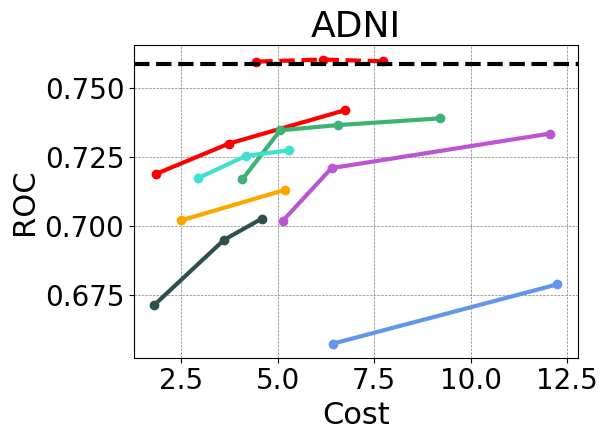
\includegraphics[width=\linewidth]{figures/adni_roc.png}
    % \caption{Synthetic}\label{fig:sub1}
  \end{subfigure}
  % ----- 2nd column -------------------------------------------------
  \begin{subfigure}[t]{.32\textwidth}
    \centering
    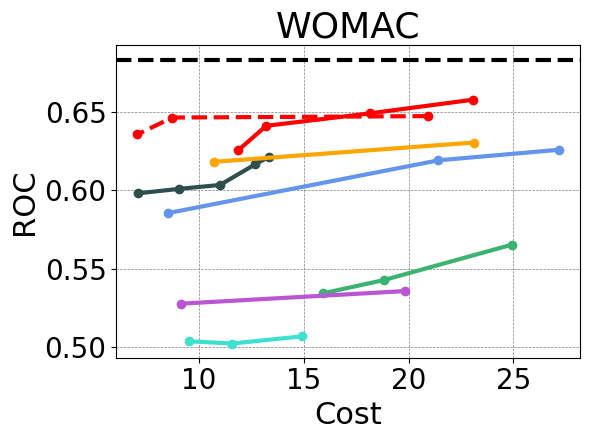
\includegraphics[width=\linewidth]{figures/womac_roc.png}
    % \caption{ADNI}\label{fig:sub2}
  \end{subfigure}
  % ----- 3rd column -------------------------------------------------
  \begin{subfigure}[t]{.32\textwidth}
    \centering
    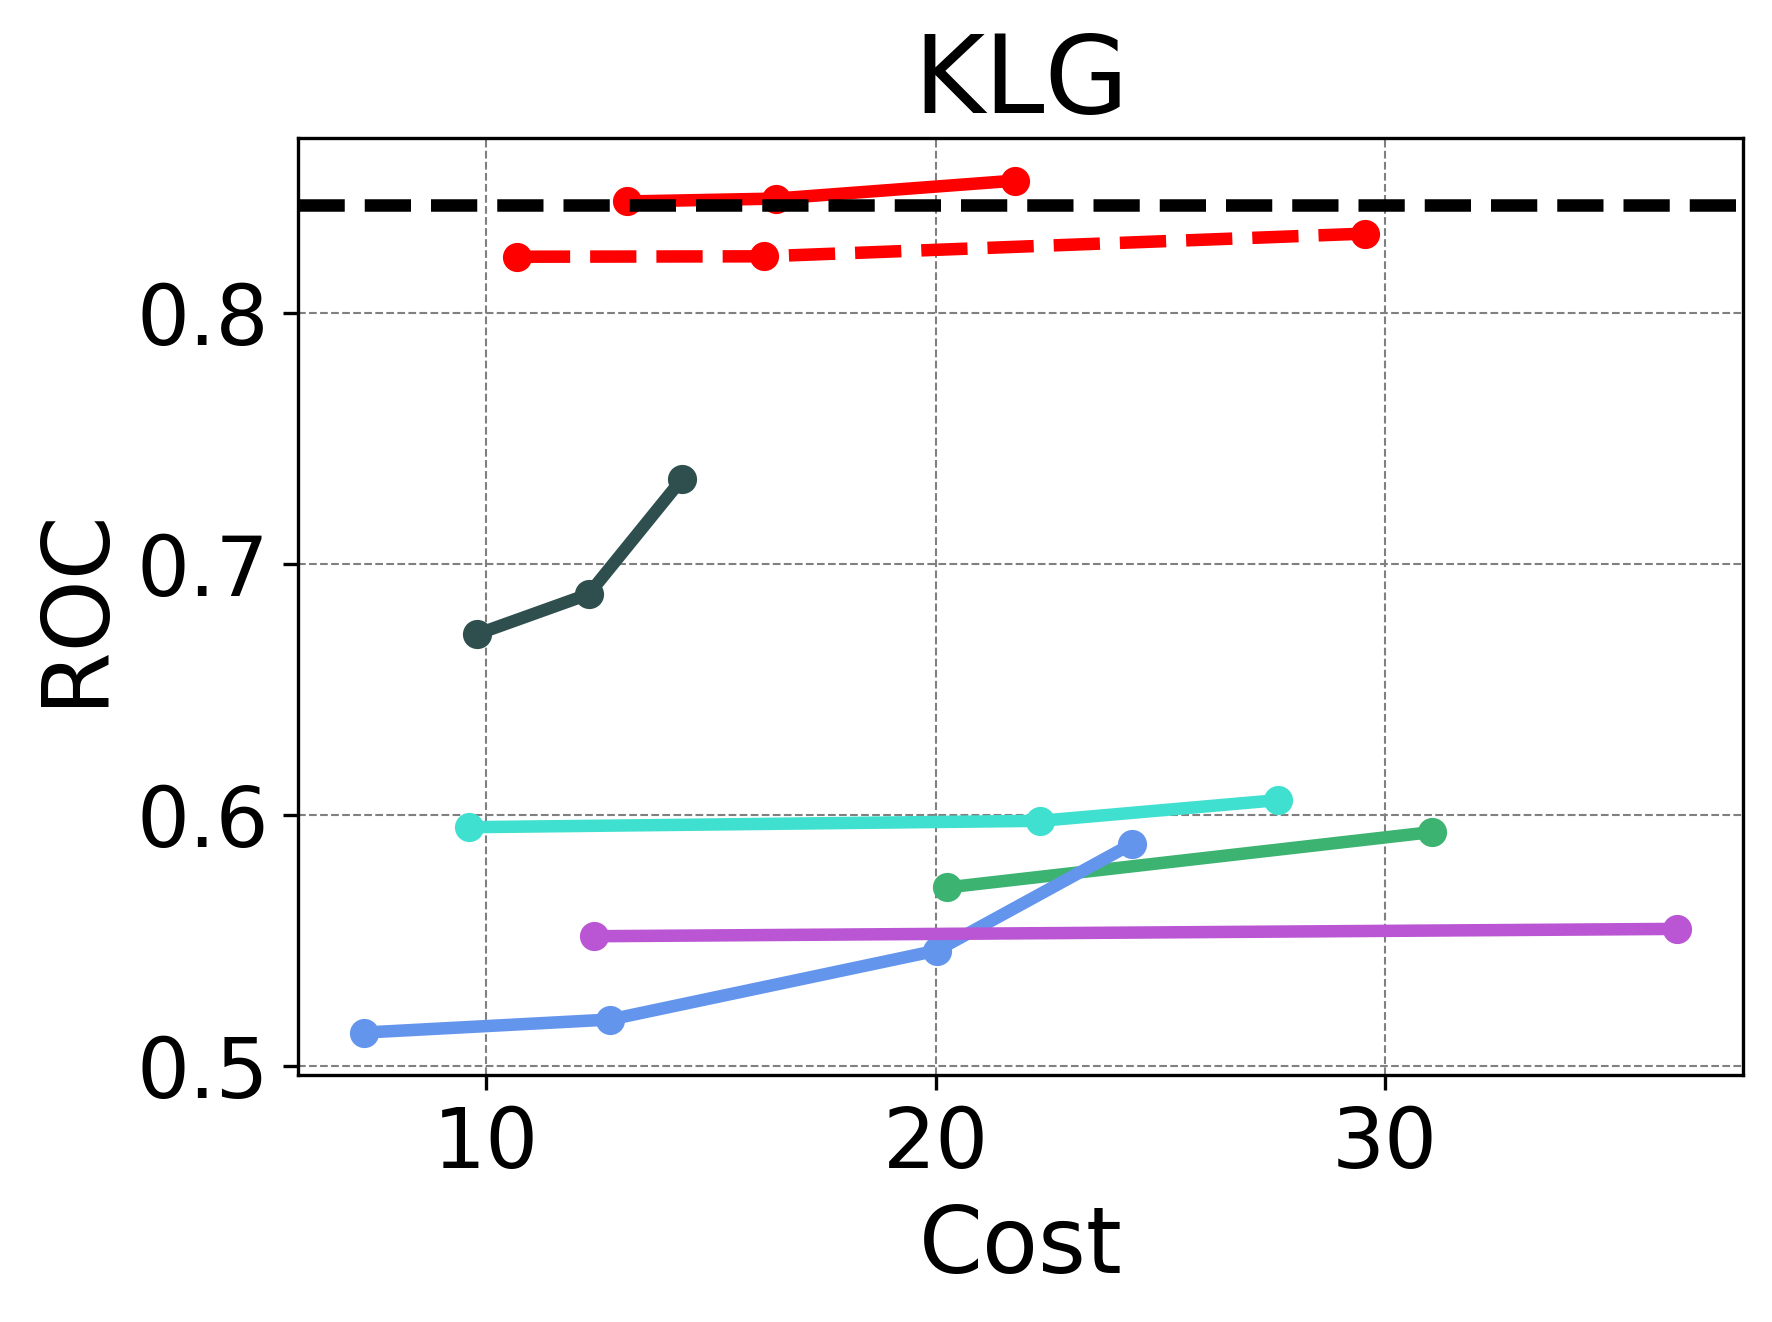
\includegraphics[width=\linewidth]{figures/klg_roc.png}
    % \caption{WOMAC}\label{fig:sub3}
  \end{subfigure}
  }
  % \par\bigskip            % vertical gap between plots and legend
  \begin{minipage}{\textwidth}
    \centering
    % trim=⟨left bottom right top⟩ clip    — remove surrounding whitespace if needed
    
\includegraphics[width=0.9\textwidth,trim=0 0 0 0,clip]{figures/legend_only.png}
  \end{minipage}
  \caption{Additional results on performance/cost of models, measured by ROC AUC across varying average acquisition budgets on real‑world datasets. Best viewed in color.}
  \label{fig:roc_auc}
\end{figure*}

\subsection{Full Results with Mean and Standard Deviation}
Tables.~\ref{tab:synthetic}, \ref{tab:adni}, \ref{tab:womac}, and \ref{tab:klg} report the mean and standard deviation for each data point presented in Figs.~\ref{fig:performance} and~\ref{fig:roc_auc}, computed over five independent runs.


\begin{table}[ht]
\captionsetup{
    % skip=10pt,
    %font=9pt,
    % labelfont=it 
}
\caption{Full results for accuracy vs. average cost on synthetic dataset.}
\label{tab:synthetic}
\vskip 0.1in
\begin{center}

\begin{sc}
\resizebox{0.5\linewidth}{!}{ 
    \begin{tabular}{c c c}
      \toprule
      \multirow{2}{*}{Method} & \multicolumn{2}{c}{Synthetic} \\ \cline{2-3}
       & Accuracy & Cost \\ \hline
      \multirow{3}{*}{ASAC}
    & $0.449\pm0.078$ & $5.803\pm5.180$ \\ 
    & $0.567\pm0.161$ & $9.929\pm8.365$ \\
    & $0.624\pm0.136$ & $11.780\pm5.211$ \\
    \hline
    
      \multirow{3}{*}{RAS}
        & $0.316\pm0.031$ & $6.390\pm5.316$ \\
        & $0.315\pm0.032$ & $6.852\pm5.129$ \\
        & $0.336\pm0.022$ & $11.003\pm2.638$ \\ \hline
      \multirow{2}{*}{AS}
        & $0.320\pm0.014$ & $9.210\pm2.344$ \\
        & $0.335\pm0.033$ & $12.870\pm3.762$ \\ \hline
      \multirow{3}{*}{DIME}
        & $0.497\pm0.078$ & $4.000\pm0.000$ \\
        & $0.501\pm0.080$ & $4.662\pm0.557$ \\
        & $0.509\pm0.084$ & $5.375\pm1.213$ \\ \hline
      \multirow{3}{*}{DiFA}
        & $0.444\pm0.015$ & $6.466\pm0.058$ \\ 
        & $0.463\pm0.017$ & $8.249\pm0.420$ \\
        & $0.504\pm0.010$ & $10.138\pm0.129$ \\
        \hline        
      \multirow{3}{*}{\texttt{NOCT-Contrastive}}
        & $0.670\pm0.002$ & $6.494\pm0.005$ \\
        & $0.815\pm0.005$ & $9.471\pm0.033$ \\
        & $0.855\pm0.002$ & $11.315\pm0.012$ \\ \hline
        
      \multirow{4}{*}{\texttt{NOCT-Amortized}}
        & $0.512\pm0.018$ & $3.580\pm0.292$ \\
        & $0.603\pm0.026$ & $6.906\pm0.174$ \\
        & $0.640\pm0.017$ & $8.6358\pm0.164$ \\
        & $0.666\pm0.006$ & $11.555\pm0.087$ \\ \bottomrule
    \end{tabular}
    }
    \end{sc}

\end{center}
% \vskip -0.1in
\vspace{-0.15in}

\end{table}

        
\begin{table}[ht]
\captionsetup{
    % skip=10pt,
    %font=9pt,
    % labelfont=it 
}
\caption{Full results for AP and ROC vs. average cost on ADNI prediction.}
\label{tab:adni}
\vskip 0.1in
\begin{center}

\begin{sc}
\resizebox{0.65\linewidth}{!}{ 
        \begin{tabular}{c c c c}
      \toprule
      \multirow{2}{*}{Method} & \multicolumn{3}{c}{ADNI} \\ \cline{2-4}
       & AP & ROC & Cost \\ \hline
      \multirow{2}{*}{ASAC}
        & $0.449\pm0.041$ & $0.657\pm0.038$ & $6.442\pm6.093$ \\ 
        & $0.497\pm0.034$ & $0.679\pm0.015$ & $12.242\pm2.648$ \\
        \hline

      \multirow{4}{*}{RAS}
        & $0.538\pm0.036$ & $0.717\pm0.024$ & $4.087\pm0.735$ \\
        & $0.567\pm0.015$ & $0.735\pm0.008$ & $5.064\pm0.324$ \\
        & $0.567\pm0.022$ & $0.737\pm0.012$ & $6.560\pm2.459$ \\
        & $0.572\pm0.012$ & $0.739\pm0.011$ & $9.197\pm1.438$ \\ \hline

      \multirow{3}{*}{AS}
        & $0.514\pm0.046$ & $0.702\pm0.038$ & $5.133\pm1.659$ \\ 
        & $0.536\pm0.021$ & $0.721\pm0.014$ & $6.394\pm2.477$ \\
        & $0.546\pm0.021$ & $0.734\pm0.013$ & $12.054\pm1.763$ \\
        \hline
      \multirow{3}{*}{DIME}
        & $0.519\pm0.037$ & $0.671\pm0.047$ & $1.801\pm0.050$ \\
        & $0.538\pm0.045$ & $0.695\pm0.048$ & $3.607\pm0.084$ \\
        & $0.544\pm0.048$ & $0.703\pm0.049$ & $4.587\pm0.330$ \\ \hline
      \multirow{3}{*}{DiFA}
        & $0.520\pm0.027$ & $0.717\pm0.029$ & $2.925\pm0.127$ \\ 
        & $0.529\pm0.025$ & $0.725\pm0.028$ & $4.180\pm0.043$ \\
        & $0.530\pm0.027$ & $0.727\pm0.033$ & $5.292\pm0.107$ \\
        \hline

      \multirow{3}{*}{\texttt{NOCT-Contrastive}}
& $0.578\pm0.004$ & $0.760\pm0.003$ & $4.434\pm0.042$ \\ 
& $0.579\pm0.009$ & $0.760\pm0.003$ & $6.164\pm0.068$ \\
& $0.584\pm0.013$ & $0.760\pm0.006$ & $7.727\pm0.094$ \\
\hline

      \multirow{3}{*}{\texttt{NOCT-Amortized}}
        & $0.548\pm0.025$ & $0.719\pm0.025$ & $1.851\pm0.019$ \\
        & $0.569\pm0.023$ & $0.730\pm0.015$ & $3.729\pm0.079$ \\
        & $0.576\pm0.021$ & $0.742\pm0.012$ & $6.743\pm0.330$ \\ \bottomrule
    \end{tabular}
    }
    \end{sc}

\end{center}
% \vskip -0.1in
\vspace{-0.15in}

\end{table}



\begin{table}[ht]
% \captionsetup{
%     % skip=2pt,
%     %font=9pt,
%     labelfont=it 
% }
\caption{Full results for AP and ROC vs. average cost on WOMAC score prediction.}
\label{tab:womac}
\vskip 0.1in
\begin{center}

\begin{sc}
\resizebox{0.67\linewidth}{!}{ 
    \begin{tabular}{c c c c}
    \toprule
    
        \multirow{2}{*}{Method} & \multicolumn{3}{c}{WOMAC} \\
        \cline{2-4}
         & AP & ROC & Cost \\
        \hline
        \multirow{3}{*}{ASAC} 
& $0.269\pm0.032$ & $0.586\pm0.060$ & $8.541\pm2.136$ \\ 
& $0.293\pm0.018$ & $0.619\pm0.028$ & $21.423\pm6.480$ \\
& $0.299\pm0.025$ & $0.626\pm0.026$ & $27.175\pm6.933$ \\
\hline

        \hline
        \multirow{3}{*}{RAS} 
& $0.226\pm0.008$ & $0.534\pm0.019$ & $15.930\pm3.475$ \\
& $0.231\pm0.007$ & $0.543\pm0.009$ & $18.810\pm1.802$ \\
& $0.251\pm0.019$ & $0.565\pm0.024$ & $24.939\pm3.796$ \\ \hline

        \multirow{2}{*}{AS} 
        & $0.225\pm0.005$ & $0.528\pm0.008$ & $9.160\pm2.271$ \\
        & $0.235\pm0.011$	 & $0.536\pm0.012$ & $19.826\pm10.326$ \\
        \hline
        \multirow{5}{*}{DIME} 
& $0.297\pm0.025$ & $0.598\pm0.043$ & $7.073\pm0.093$ \\
& $0.297\pm0.025$ & $0.601\pm0.043$ & $9.036\pm0.198$ \\
& $0.302\pm0.028$ & $0.603\pm0.044$ & $11.009\pm0.310$ \\
& $0.305\pm0.027$ & $0.617\pm0.037$ & $12.696\pm0.357$ \\
& $0.310\pm0.028$ & $0.621\pm0.038$ & $13.325\pm0.643$ \\ \hline
        \multirow{3}{*}{DiFA} 
& $0.199\pm0.009$ & $0.504\pm0.004$ & $9.532\pm0.091$ \\
& $0.211\pm0.005$ & $0.502\pm0.002$ & $11.584\pm0.630$ \\
& $0.217\pm0.004$ & $0.507\pm0.008$ & $14.936\pm1.433$ \\ \hline


        \multirow{3}{*}{\texttt{NOCT-Contrastive}} 
& $0.317\pm0.003$ & $0.636\pm0.0012$ & $7.063\pm0.004$ \\ 
& $0.328\pm0.004$ & $0.646\pm0.003$ & $8.729\pm0.011$ \\
& $0.339\pm0.008$ & $0.647\pm0.003$ & $20.921\pm0.058$ \\
\hline



        \multirow{4}{*}{\texttt{NOCT-Amortized}} 
& $0.311\pm0.007$ & $0.625\pm0.006$ & $11.862\pm0.074$ \\
& $0.327\pm0.020$ & $0.641\pm0.018$ & $13.212\pm0.180$ \\
& $0.335\pm0.015$ & $0.649\pm0.015$ & $18.178\pm0.082$ \\
& $0.340\pm0.013$ & $0.658\pm0.011$ & $23.061\pm0.059$ \\ \bottomrule

    \end{tabular}
    }
    \end{sc}

\end{center}
% \vskip -0.2in
\vspace{-0.13in}
\end{table}


\begin{table}[ht]
\captionsetup{
    % skip=10pt,
    %font=9pt,
    % labelfont=it 
}
\caption{Full results for AP and ROC vs. average cost on KLG prediction.}
\label{tab:klg}
\vskip 0.1in
\begin{center}

\begin{sc}
\resizebox{0.67\linewidth}{!}{ 
    \begin{tabular}{cccc}
    \toprule
        \multirow{2}{*}{Method} & \multicolumn{3}{c}{KLG} \\
        \cline{2-4}
         & AP & ROC & Cost \\
        \hline
        \multirow{4}{*}{ASAC} 
& $0.258\pm0.021$ & $0.513\pm0.035$ & $7.284\pm4.694$ \\ 
& $0.266\pm0.018$ & $0.519\pm0.019$ & $12.756\pm6.584$ \\
& $0.283\pm0.009$ & $0.546\pm0.024$ & $20.025\pm6.504$ \\
& $0.304\pm0.008$ & $0.589\pm0.015$ & $24.361\pm15.940$ \\
\hline

        
        \hline
        \multirow{2}{*}{RAS} 
        & $0.290\pm0.012$ & $0.571\pm0.023$ & $20.253\pm11.269$ \\
        & $0.313\pm0.049$ & $0.593\pm0.063$ & $31.044\pm8.560$ \\
        \hline
        \multirow{2}{*}{AS} 
        & $0.277\pm0.012$ & $0.552\pm0.021$ & $12.394\pm2.027$ \\
        & $0.285\pm0.022$ &$0.555\pm0.015$  & $36.499\pm8.124$ \\
        \hline
        \multirow{3}{*}{DIME} 
& $0.418\pm0.016$ & $0.672\pm0.023$ & $9.787\pm0.040$ \\
& $0.438\pm0.018$ & $0.688\pm0.028$ & $12.281\pm0.005$ \\
& $0.486\pm0.026$ & $0.734\pm0.024$ & $14.359\pm0.148$ \\ \hline
        \multirow{3}{*}{DiFA} 
& $0.310\pm0.006$ & $0.595\pm0.019$ & $9.611\pm1.743$ \\ 
& $0.322\pm0.011$ & $0.598\pm0.015$ & $22.331\pm3.465$ \\
& $0.336\pm0.010$ & $0.606\pm0.013$ & $27.615\pm6.411$ \\
\hline

        \multirow{3}{*}{\texttt{NOCT-Contrastive}} 
& $0.644\pm0.003$ & $0.822\pm0.001$ & $10.687\pm0.018$ \\ 
& $0.649\pm0.002$ & $0.822\pm0.002$ & $16.192\pm0.062$ \\
& $0.663\pm0.004$ & $0.831\pm0.001$ & $29.546\pm0.052$ \\
\hline

        \multirow{3}{*}{\texttt{NOCT-Amortized}} 
& $0.641\pm0.054$ & $0.844\pm0.020$ & $13.144\pm0.107$ \\
& $0.639\pm0.056$ & $0.845\pm0.022$ & $16.448\pm0.228$ \\
& $0.655\pm0.042$ & $0.853\pm0.017$ & $21.776\pm0.323$ \\ \bottomrule

    \end{tabular}
    }
    \end{sc}

\end{center}
% \vskip -0.1in
\vspace{-0.15in}

\end{table}


\end{document}
